\chapter{Global Event Reconstruction}

In the previous chapter, we discussed the interactions of particles with the individual subdetectors and how these generate electrical signals.
Now, we shall discuss the reverse process, namely reconstructing the individual particles or physics objects from the electrical signals recorded by the subdetectors.

Traditionally, each class of physics object was reconstructed using information from a single subdetector: muons from the muon chambers, isolated photons and electrons from the ECAL, jets and missing transverse energy from the HCAL, and secondary vertices from $\tau$ lepton and $b$ quark decays from the tracker.
However, as depicted in Figure~\ref{fig:cms_slice}, each type of particle interacts with multiple different subdetectors and this information is lost unless the information from all the subdetectors is combined into a single global event description.

The particle flow (PF) algorithm leverages the fine angular granularity of the calorimeters and the excellent momentum resolution of the inner tracker and muon chambers to greatly improve the reconstruction of physics objects and include soft particles that would otherwise be ignored.
This is especially advantageous for jet energy measurements as roughly 62\% of the jet energy is carried by charged hadrons, approximately 27\% by photons, around 10\% by neutral hadrons, and about 1.5\% by neutrinos.

\begin{figure}[htbp]
  \begin{center}
    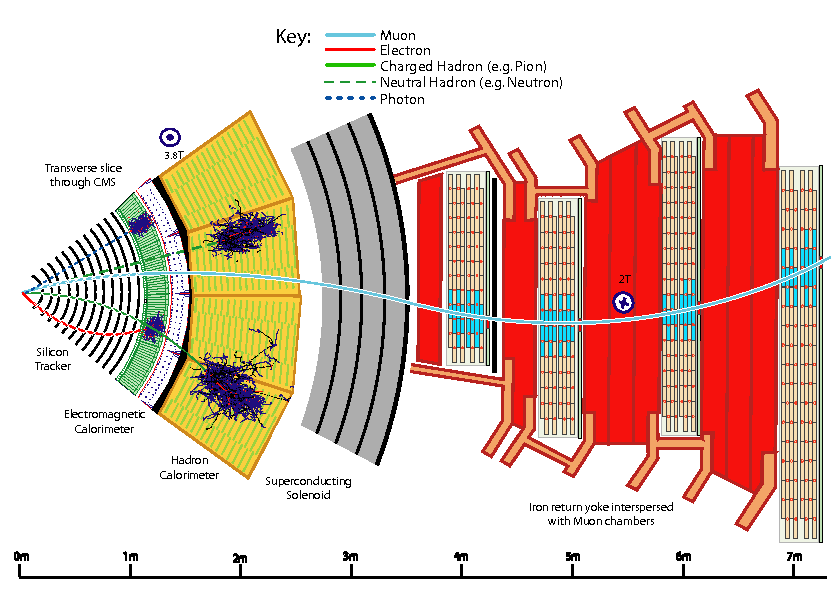
\includegraphics[width=0.875\textwidth]{Reconstruction/Figures/cms_slice.png}
    \caption{
      A sketch of a transverse slice of the CMS detector showing particle interactions from the interaction point to the muon detector.
      % Charge particles tracks are shown with solid lines while the paths of neutral particles are shown with dotted lines. 
      % The muon and charged pion are positively charged and the electron is negatively charged.
      % Neutrinos do not interact with the detector at an appreciably rate.
      Reprinted from Reference~\cite{}. % https://iopscience.iop.org/article/10.1088/1748-0221/12/10/P10003/meta
    }
    \label{fig:cms_slice}
  \end{center}
\end{figure}

The distinguishing feature of the PF algorithm is to combine multiple detector signals together into a single PF candidate.
The input detector signals are the tracks, vertices, calorimeter clusters, and muon segments described in Section~\ref{sec:pf_elements}.
Based on their proximity in the $\eta$-$\phi$, these PF elements are combined into muons, electrons, and hadrons.
Muon segments are combined with inner tracks to produce muons, inner tracks are combined with calorimeter clusters to produce electrons and charge hadrons, and calorimeter clusters are correlated to produce photons and neutral hadrons.

The PF algorithm reconstructs particles in the blocks described in Section~\ref{sec:pf_cands} and after each block any PF elements associated to a PF candidate are not considered by the following blocks.
For example, clusters associated with photons will not be used when reconstructing neutral hadrons.
After all PF candidates are identified, they can be combined into event-wide variables such as jets and the missing transverse energy as described in Section~\ref{sec:pf_event}. 

\section{Particle Flow Elements}
\label{sec:pf_elements}

\subsection{Tracks}
\label{sec:pf_tracks}

Some text.

\subsection{Primary Vertexing}
\label{sec:pf_pv}

\subsection{Secondary Vertexing}
\label{sec:pf_csv}

\subsection{Calorimeter Clusters}
\label{sec:pf_clusters}

\section{Particle Identification}
\label{sec:pf_cands}

\subsection{Muons}
\label{sec:pf_muons}

\subsection{Electrons and Isolated Photons}
\label{sec:pf_egamma}

\subsection{Hadrons and Nonisolated Photons}
\label{sec:pf_hadrons}

\section{Event Variables}
\label{sec:pf_event}

\subsection{Jets}
\label{sec:pf_jets}

\subsection{Missing Tranverse Energy}
\label{sec:pf_met}

\iffalse
\section{Analysis Selections}
\label{sec:ana_sel}

\subsection{Photons}
\label{sec:ana_photons}

We select high-\ET\ photons from the ECAL Barrel. First, we apply the following cuts to select high-\ET\ photon candidates:
\begin{itemize}
\item Super cluster $\ET > 175\GeV$
\item Super cluster $\abs\eta < 1.4442$ .
\end{itemize}
We use the uncorrected \ET\ of the supercluster as photon \ET. 
The use of supercluster raw \ET\ is motivated by an observation that this energy correction causes photon objects with large cluster shower width to exhibit unphysical energies. 
Figure~\ref{fig:corr_vs_sieie} is a profile of the magnitude of the energy correction in bins of \sieie. 
As an illustration, an unphysically large correction is causing the transverse momentum of the photon object in the event shown in Fig.~\ref{fig:badcorr_evtdisp} to be nearly twice as large as the \met, which is supposed to balance the visible, \ie, photon momentum. 
Photon objects with wide showers are used to estimate the hadron-to-photon misidentification background, while the photon energy resolution has an insignificant effect. 
Therefore, unbiased supercluster energy was chosen over the corrected photon energy.

\begin{figure}[htbp]
  \begin{center}
    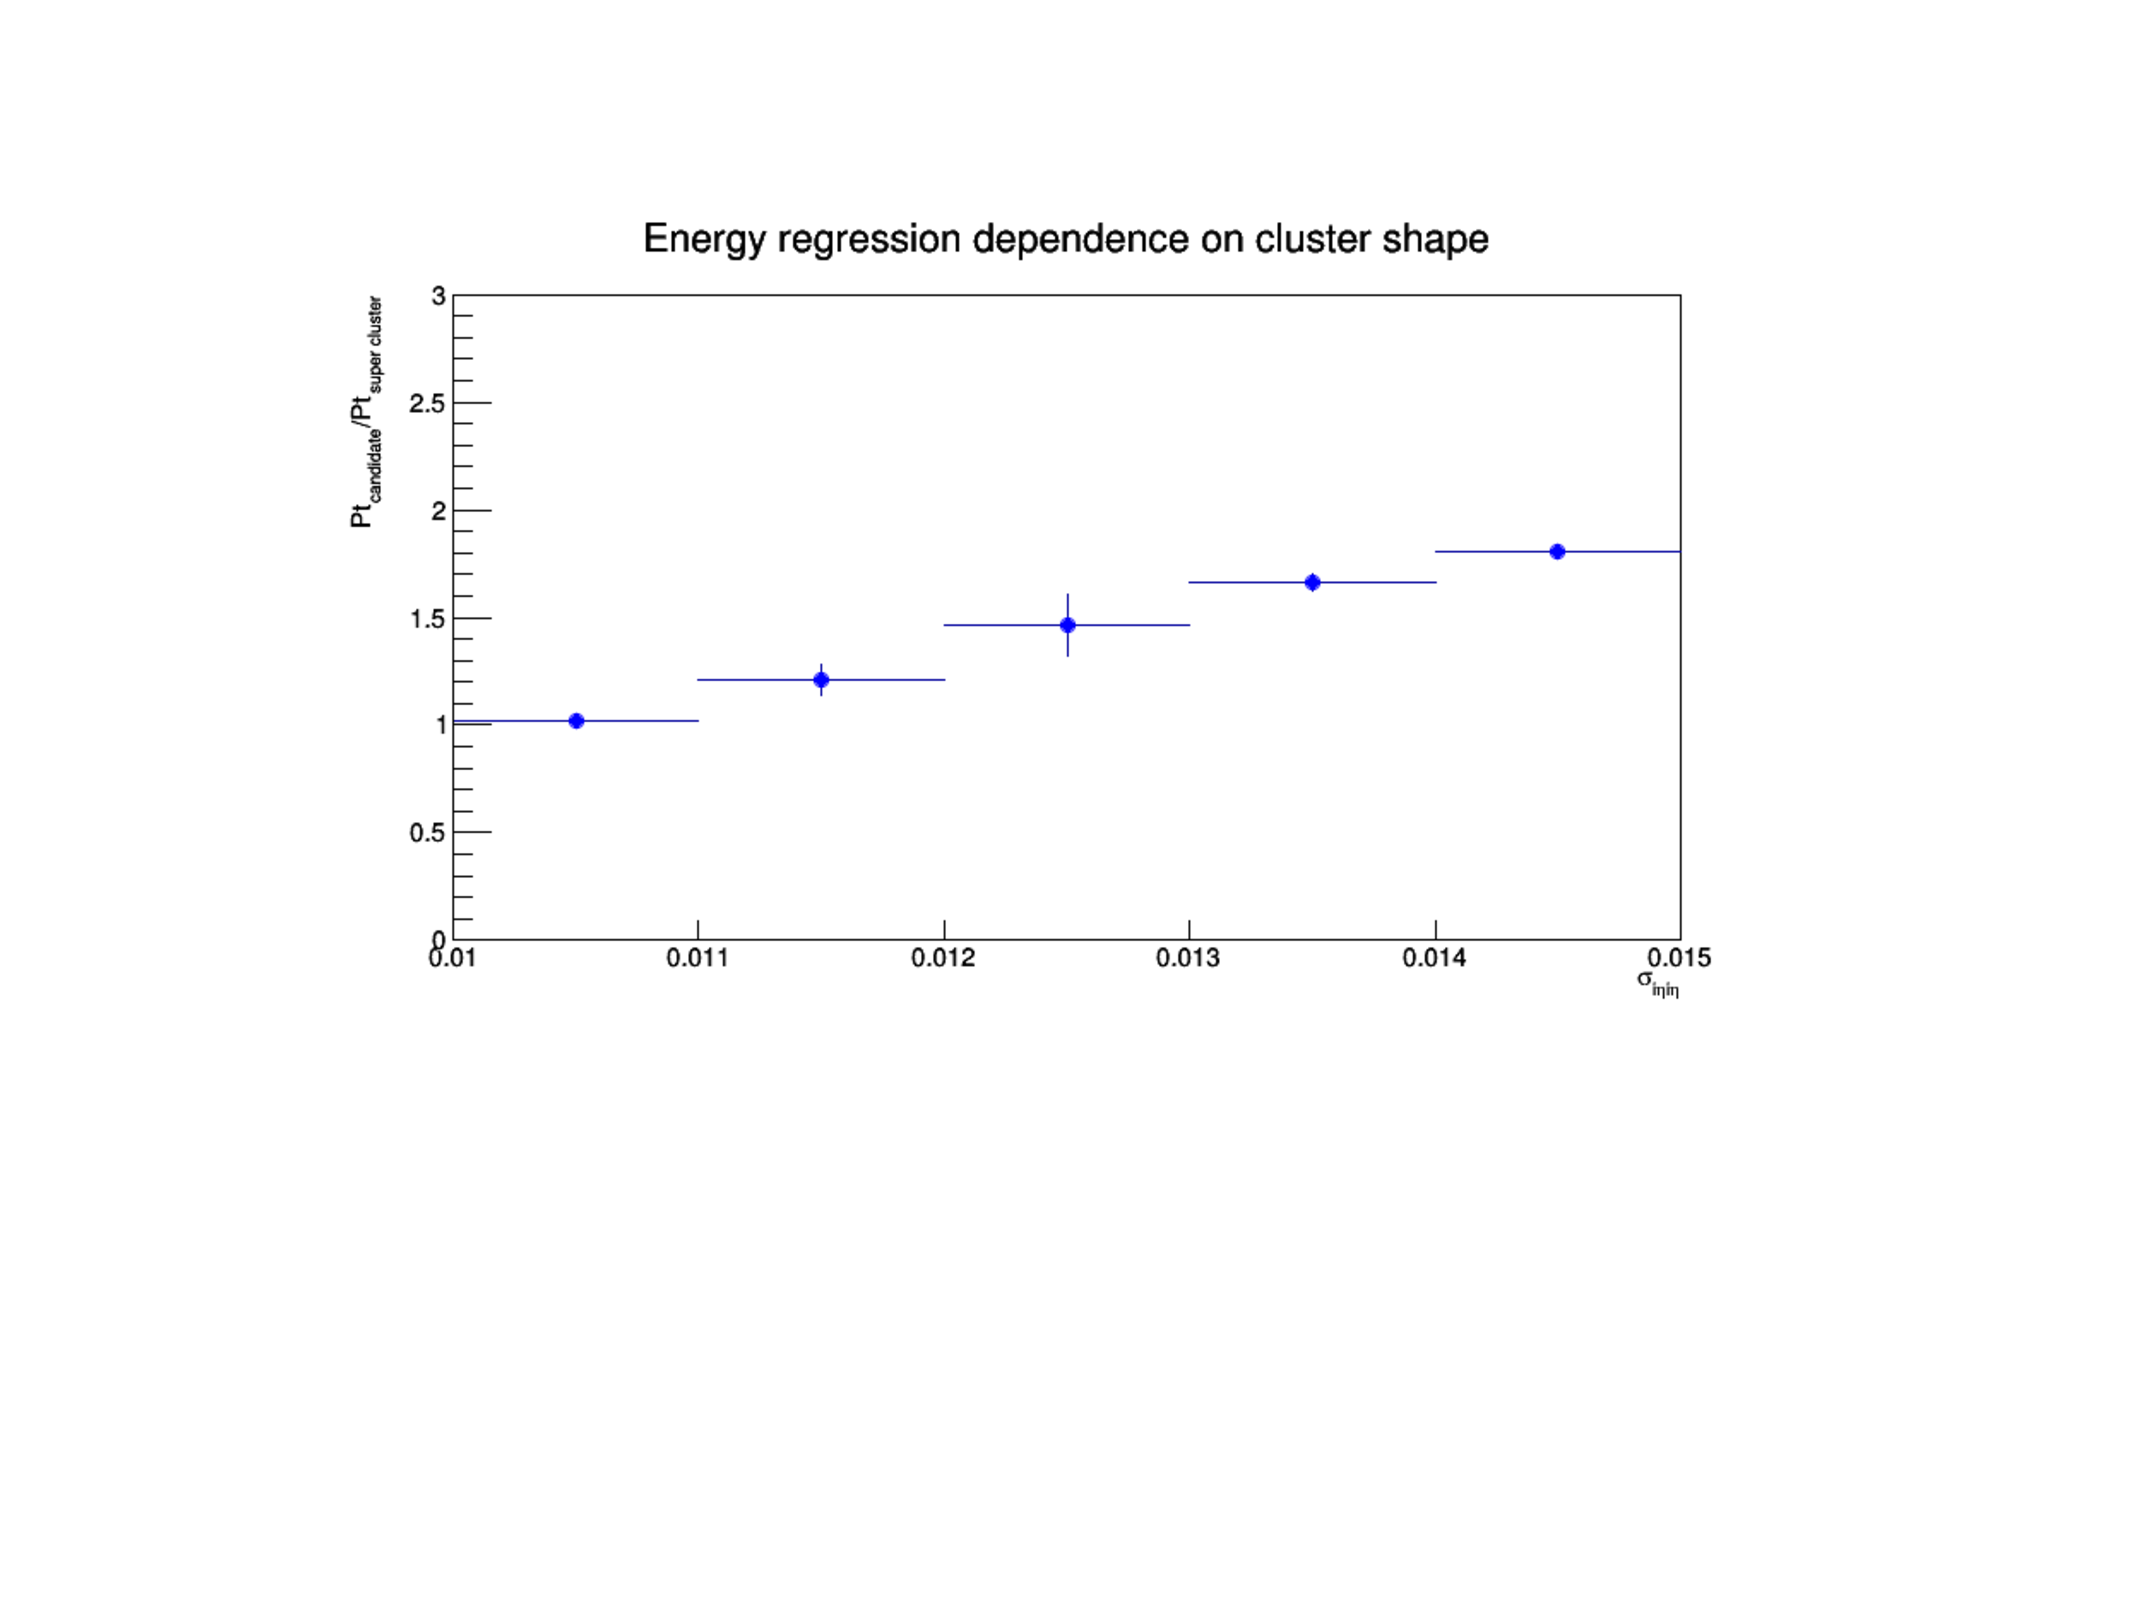
\includegraphics[width=0.6\textwidth]{Reconstruction/Figures/corr_vs_sieie.pdf}
    \caption{
      Magnitude of the energy correction on the photon object in bins of \sieie.
    }
    \label{fig:corr_vs_sieie}
  \end{center}
\end{figure}

\begin{figure}[htbp]
  \begin{center}
    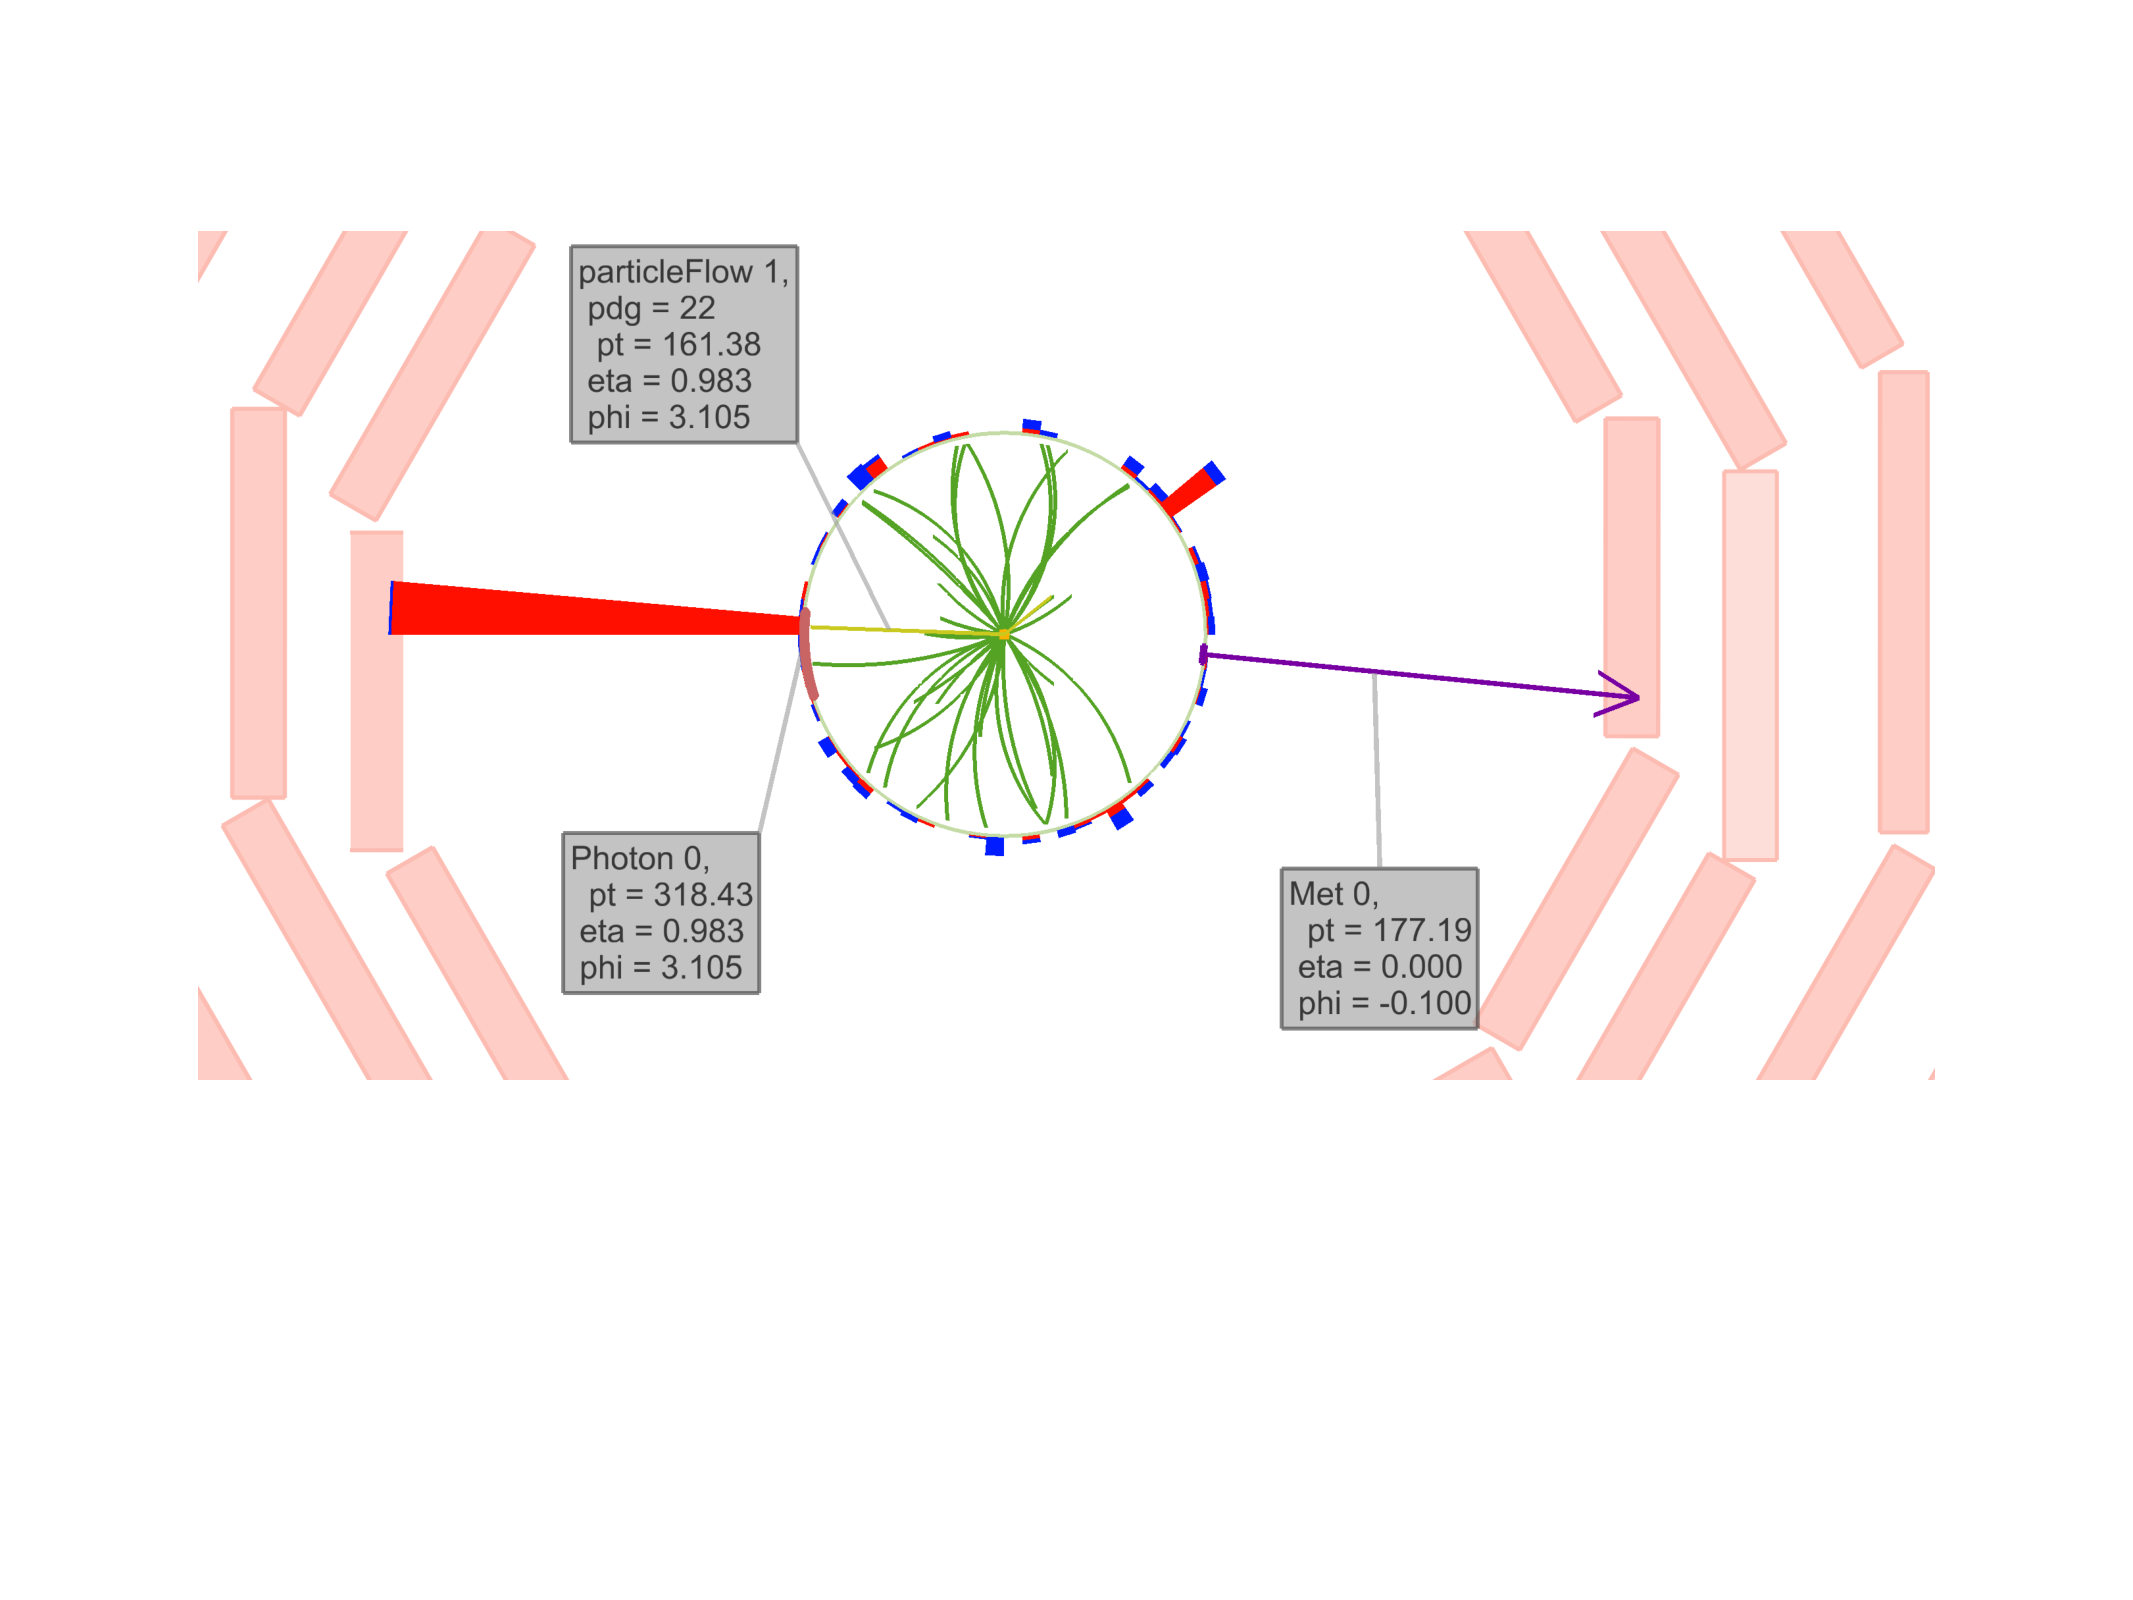
\includegraphics[width=0.6\textwidth]{Reconstruction/Figures/badcorr_evtdisp.pdf}
    \caption{
      An example event where a photon with a wide shower receives a large energy correction.
    }
    \label{fig:badcorr_evtdisp}
  \end{center}
\end{figure}

To reduce hadron-to-photon misidentification rate, we apply the following collection of isolation and shower shape cuts, which will hereby be referred to as the \egamma\ ID:
\begin{itemize}
  \item $H/E < 0.0260$
  \item $\sieie < 0.01040$
  \item $\rho$-corrected maximum PF charged hadron isolation $\ICHmax < 1.146\GeV$
  \item $\rho$-corrected PF neutral hadron isolation $\INH < 2.792\GeV + 0.0112 \times \ETg + 0.000028 \times \left(\ETg \right)^2/\GeV$
  \item $\rho$-corrected PF photon isolation $\Ig < 2.176\GeV + 0.0043 \times \ETg$
\end{itemize}

In the identification criteria, the maximum PF charged hadron isolation \ICHmax\ is the maximum of the standard PF charged hadron isolation computed for all reconstructed vertices. 
Standard PF charged hadron isolation is computed with respect to the primary vertex. 
Since the object with the highest \pt\ in the selected events is typically a photon, which has no intrinsic association to a vertex, it is possible that the identified primary vertex does not correspond to the \Pp\Pp\ interaction from which the photon object originate. 
In such cases, the photon object can be surrounded by charged hadrons, \ie, a part of a jet, and still appear isolated under the standard charged hadron isolation. 
The use of maximum isolation is a conservative measure to address such misidentification.

Effective areas for isolations are also recomputed to maintain flat pileup dependence as given in Table~\ref{tab:ea}
%
\begin{table}[htbp]
  \begin{center}
    \caption{Effective areas for isolations.} 
    \label{tab:ea}
    \begin{tabular}{|c|c|c|}
      \hline
      Isolation & $\abs\eta < 1.0$ & $1.0 < \abs\eta < 1.479$  \\
      \hline
      maximum PF charged hadron isolation & 0.01064& 0.1026 \\
      PF neutral hadron isolation & 0.0597 & 0.0807 \\
      PF photon isolation & 0.1210 & 0.1107 \\
      \hline
    \end{tabular}
  \end{center}
\end{table}

To reject electrons from the candidate sample, we require that no electron track seeds can be associated to the super cluster. This is known as the pixel seed veto.

To clean the candidate sample from photon objects originating from non-collision sources. we apply the following collection of cuts, which combined with the pixel seed veto constitutes the \Pgg-specific ID:
\begin{itemize} 
  \item Beam halo tagger $\emip < 4.9\GeV$
  \item $\sieie > 0.001$
  \item $\sipip > 0.001$
  \item Cluster seed time $\abs\tseed < 3\ns$ .
\end{itemize}
Beam halo tagger is the total energy deposited in ECAL by a hypothetical beam halo muon that passes through the photon cluster. 
Lower bounds for \sieie\ and \sipip\ as well as the requirement on the cluster seed time are employed to reject spurious photon objects arising from ``ECAL spikes'', or anomalous electronic signal induced at the ECAL Barrel photodetectors by nuclear or ionizing interactions in the photocathode.

\subsection{Electrons}
\label{sec:ana_electrons}

Electrons must have $\pt^{\Pe} > 10\GeV$ and $\abs{\eta^{\Pe}} < 2.5$ to be considered.
Additionally, electrons must pass further cuts on the following observables:
\begin{itemize}
  \item the \sieie\ of the corresponding SC,
  \item the \deta\ and \dphi\ between the SC seed crystal and the GSF track at the PV,
  \item $H/E$ of the corresponding ECAL and HCAL towers,
  \item the relative combined PF Isolation $(\ICH + \INH + \Ig) / \pt^{\Pe}$,
  \item the difference in energy measured in the tracker and the calorimeter $\abs{1/E - 1/p}$,
  \item the number of missing hits in the inner tracker,
  \item and the existence of a pair of tracks originating at a displaced vertex, indicting photon conversion.
\end{itemize}
The exact values of the cuts are tuned based on whether the electron is in the barrel or the endcap and to give desired signal efficiencies and background acceptance.
The loose ID is tuned to 90\% signal efficiency and 0.5\% background acceptance, while the tight ID is tuned to 70\% signal efficiency and 0.1\% background acceptance.

\subsection{Muons}
\label{sec:ana_muons}

Muons must have $\pt^{\Pgm} > 10\GeV$ and $\abs{\eta^{\Pgm}} < 2.5$ to be considered.
The veto muon ID is simply the requirement that a PF muon also be a Global muon, e.g., that the muon is linked between a muon signature from the inner tracker and the outer muon chambers.
The loose muon ID adds the requirement that the relative combined PF Isolation $(\ICH + \INH + \Ig) / \pt^{\Pgm}$ must be less than 0.25.
In order for a muon to pass the tight ID, it must satisfy the following additional requirements:
\begin{itemize}
   \item $\pt^{\Pgm} > 30\GeV$
   \item Relative combined PF Isolation $(\ICH + \INH + \Ig) / \pt^{\Pgm} < 0.15$ . 
   \item $\chi^2$/ndof of the global-muon track fit < 10,
   \item At least one muon-chamber hit included in the global-muon track fit,
   \item Muon segments in at least two muon stations,
   \item The corresponding racker track has transverse impact parameter $d_0 < 2\mm$ with respects to the primary vertex,
   \item The longitudinal distance of the tracker track with respects to the primary vertex is $d_z < 5\mm$,
   \item At least one pixel hit,
   \item and more than five tracker layers with hits.

\end{itemize}

\subsection{Jets}
\label{sec:ana_jets}

\section{Sources of Spurious Photons and \met}
\label{sec:issues}

\subsection{ECAL gain-switch effect}
\label{sec:gainswitch}

\begin{figure}[htbp]
  \centering
  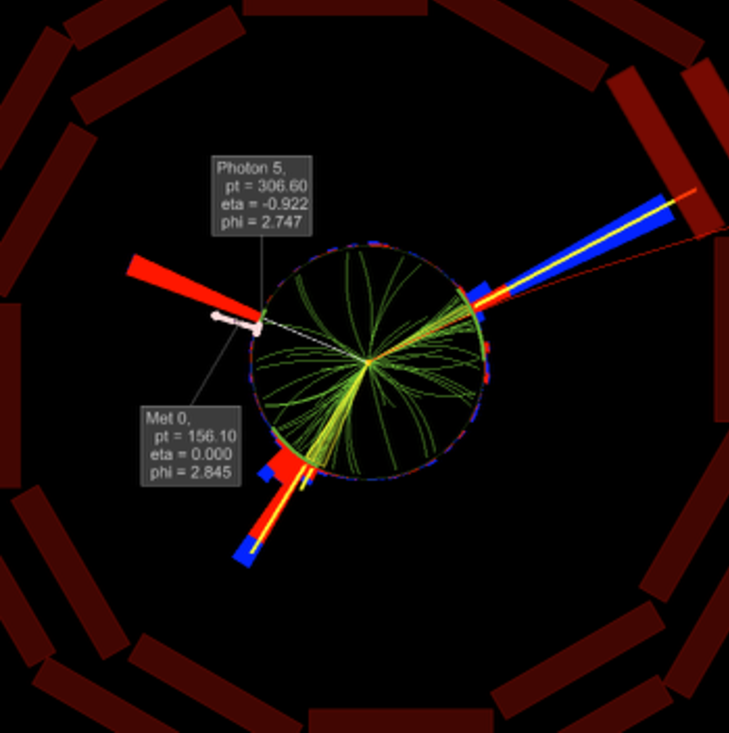
\includegraphics[width=0.48\linewidth]{Reconstruction/Figures/gsfix/evdisp_before.pdf}
  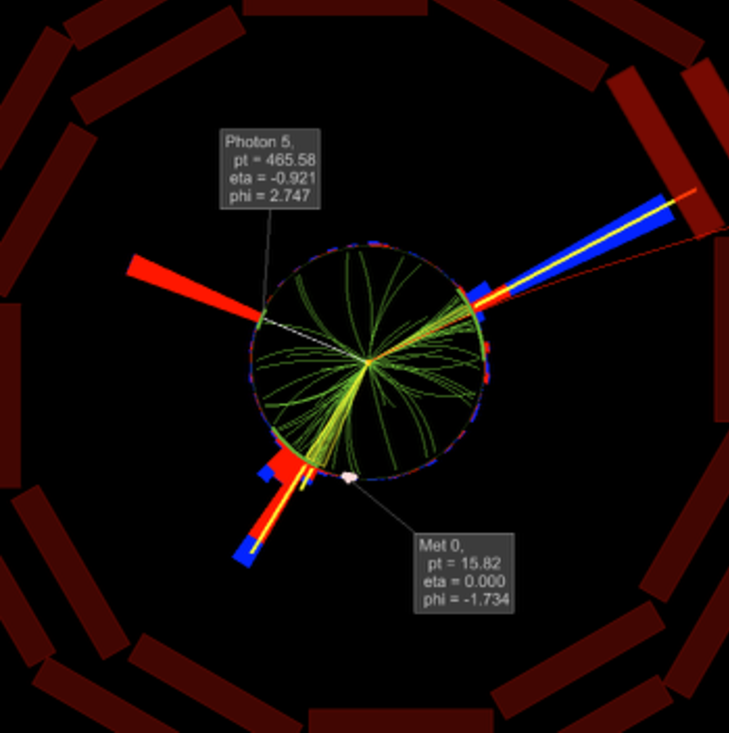
\includegraphics[width=0.48\linewidth]{Reconstruction/Figures/gsfix/evdisp_after.pdf}
  \caption{
    Two event displays comparing the same event, reconstructed without (left) and with (right) the fix for ECAL gain-switch effect.
  }
  \label{fig:eventdisplay_gsfix}
\end{figure}

The ``multi-fit'' algorithm for ECAL hit reconstruction was found to have an unexpected behavior when there is a large energy deposit onto a single ECAL crystal, such that the electronic signal converted at the frontend electronics is sourced partially from channels of the preamplifier with lower gains (6 or 1) than the default (12) channel. 
In the most dramatic cases, pulse misreconstruction would result in underestimation by hundreds of \GeV of photon \pt. 
This effect is mitigated in the reprocessed data set used for this analysis by identifying ECAL clusters whose seed crystal hit had a switch of gains, and performing an alternative pulse reconstruction when possible.

\begin{figure}[htbp]
  \centering
  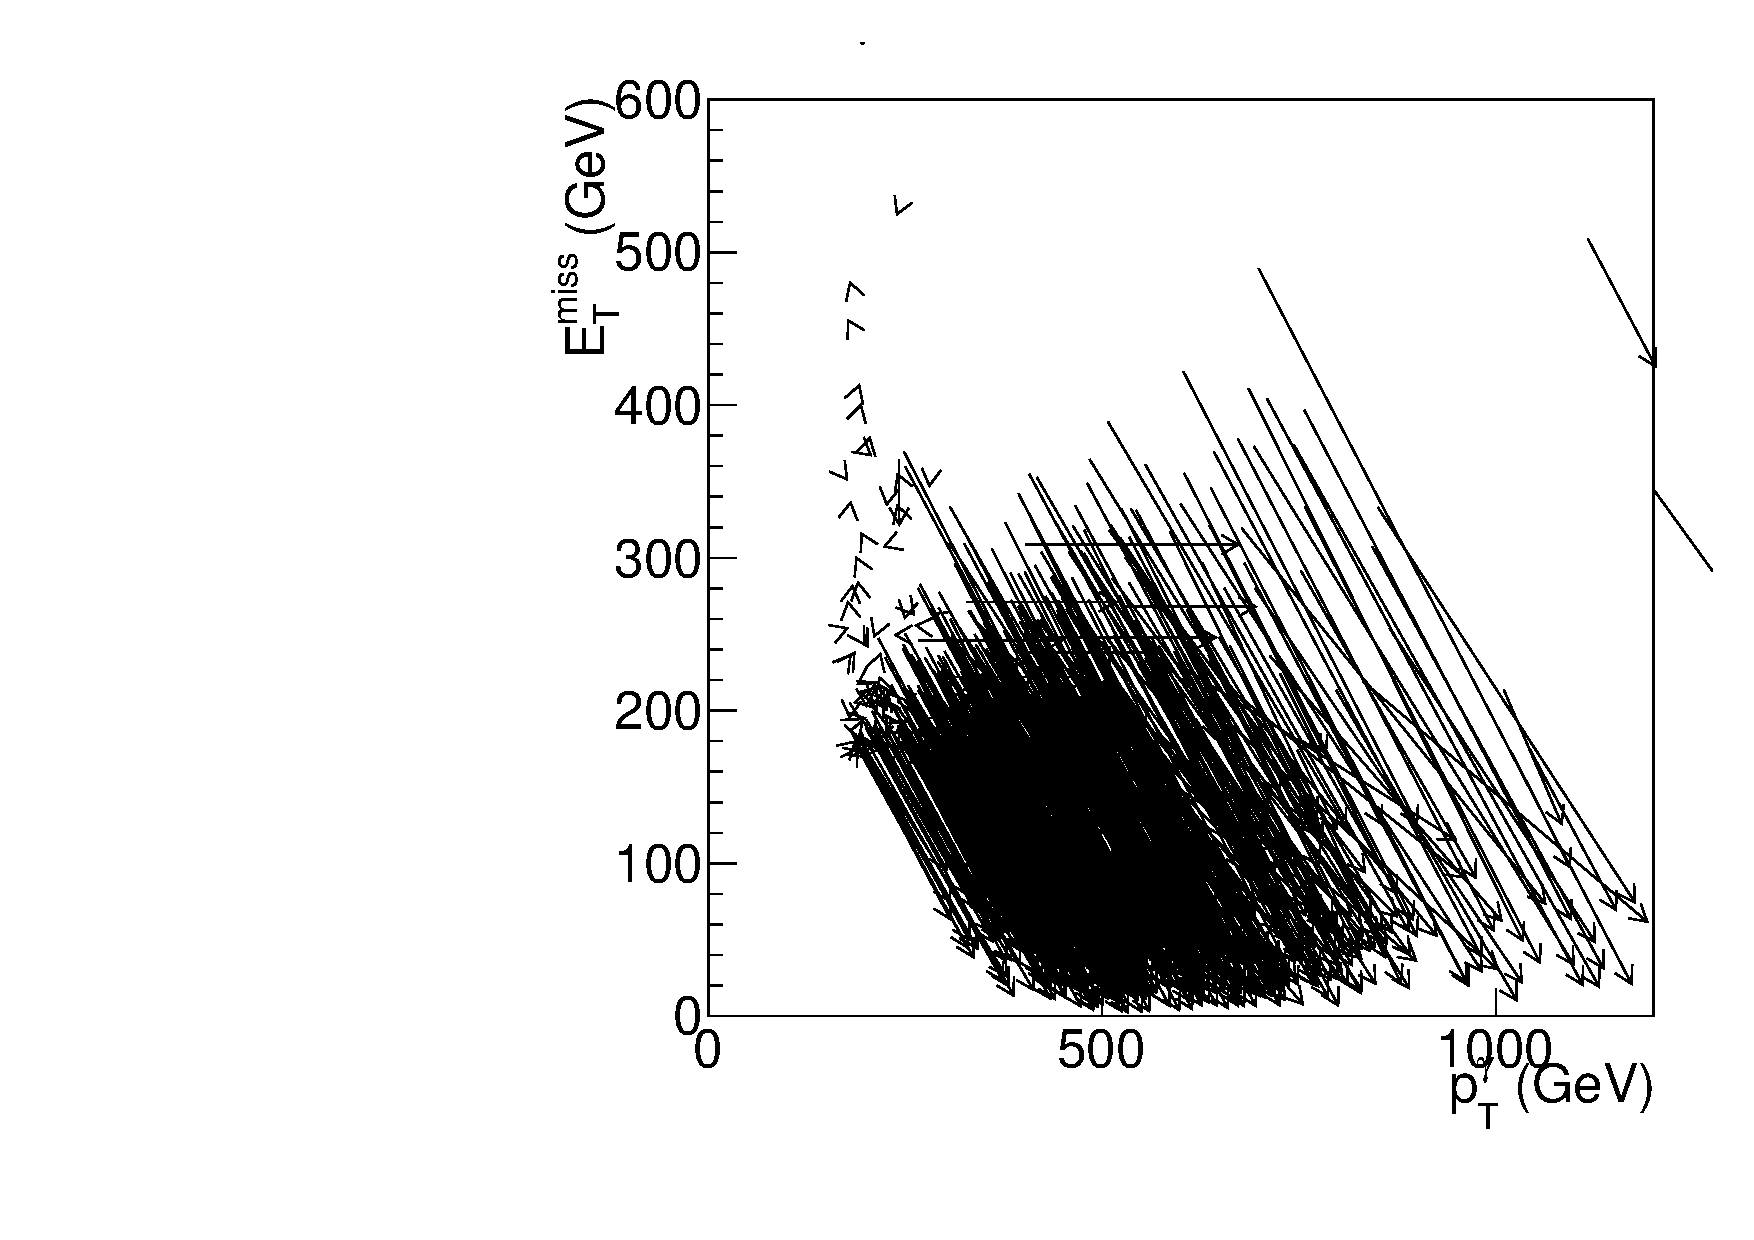
\includegraphics[width=0.48\linewidth]{Reconstruction/Figures/gsfix/movements.pdf}
  \caption{
    The change in reconstructed photon \pt\ and \met\ for events in the bin $\dphigmet < 0.05$ of the distribution in Figure~\ref{fig:dphigmet_beforegsfix}. 
    Each arrow represents a single event, the the tail (head) of the arrow corresponding to (\ETg, \met) coordinates in the datasets without (with) the fix for the gain-switch problem.
  }
  \label{fig:ptshift_gsfix}
\end{figure}

The gain-switch problem affected the analyses documented in this thesis, since large underestimation of the energy of a photon in an otherwise typical \gj\ event would introduce large missing transverse momentum to the event, typical collinear to the affected photon. 
Figures~\ref{fig:eventdisplay_gsfix} and \ref{fig:ptshift_gsfix} are the visualization of how the new dataset changes the reconstructed photon energy and \met.

\subsection{Beam Halo Phenomenology}
\label{sec:halo}

Bremsstrahlung photons emitted by beam halo muons in the ECAL volume generate a physical EM shower in the ECAL crystals. 
Large deposits energy are rare, but the rate of beam halo penetration during the 2016 run was substantial. 
The characteristic features of a shower caused by a halo particle include coincident hits in the barrel muon system and a ``trail'' of low-energy clusters in ECAL along the particle trajectory. 
The beam halo MET filter described in Section~\ref{sec:met} exploits the former, while the \emip\ variable described in Section~\ref{sec:photons} captures the latter.

\begin{figure}[tbp]
  \begin{center}
    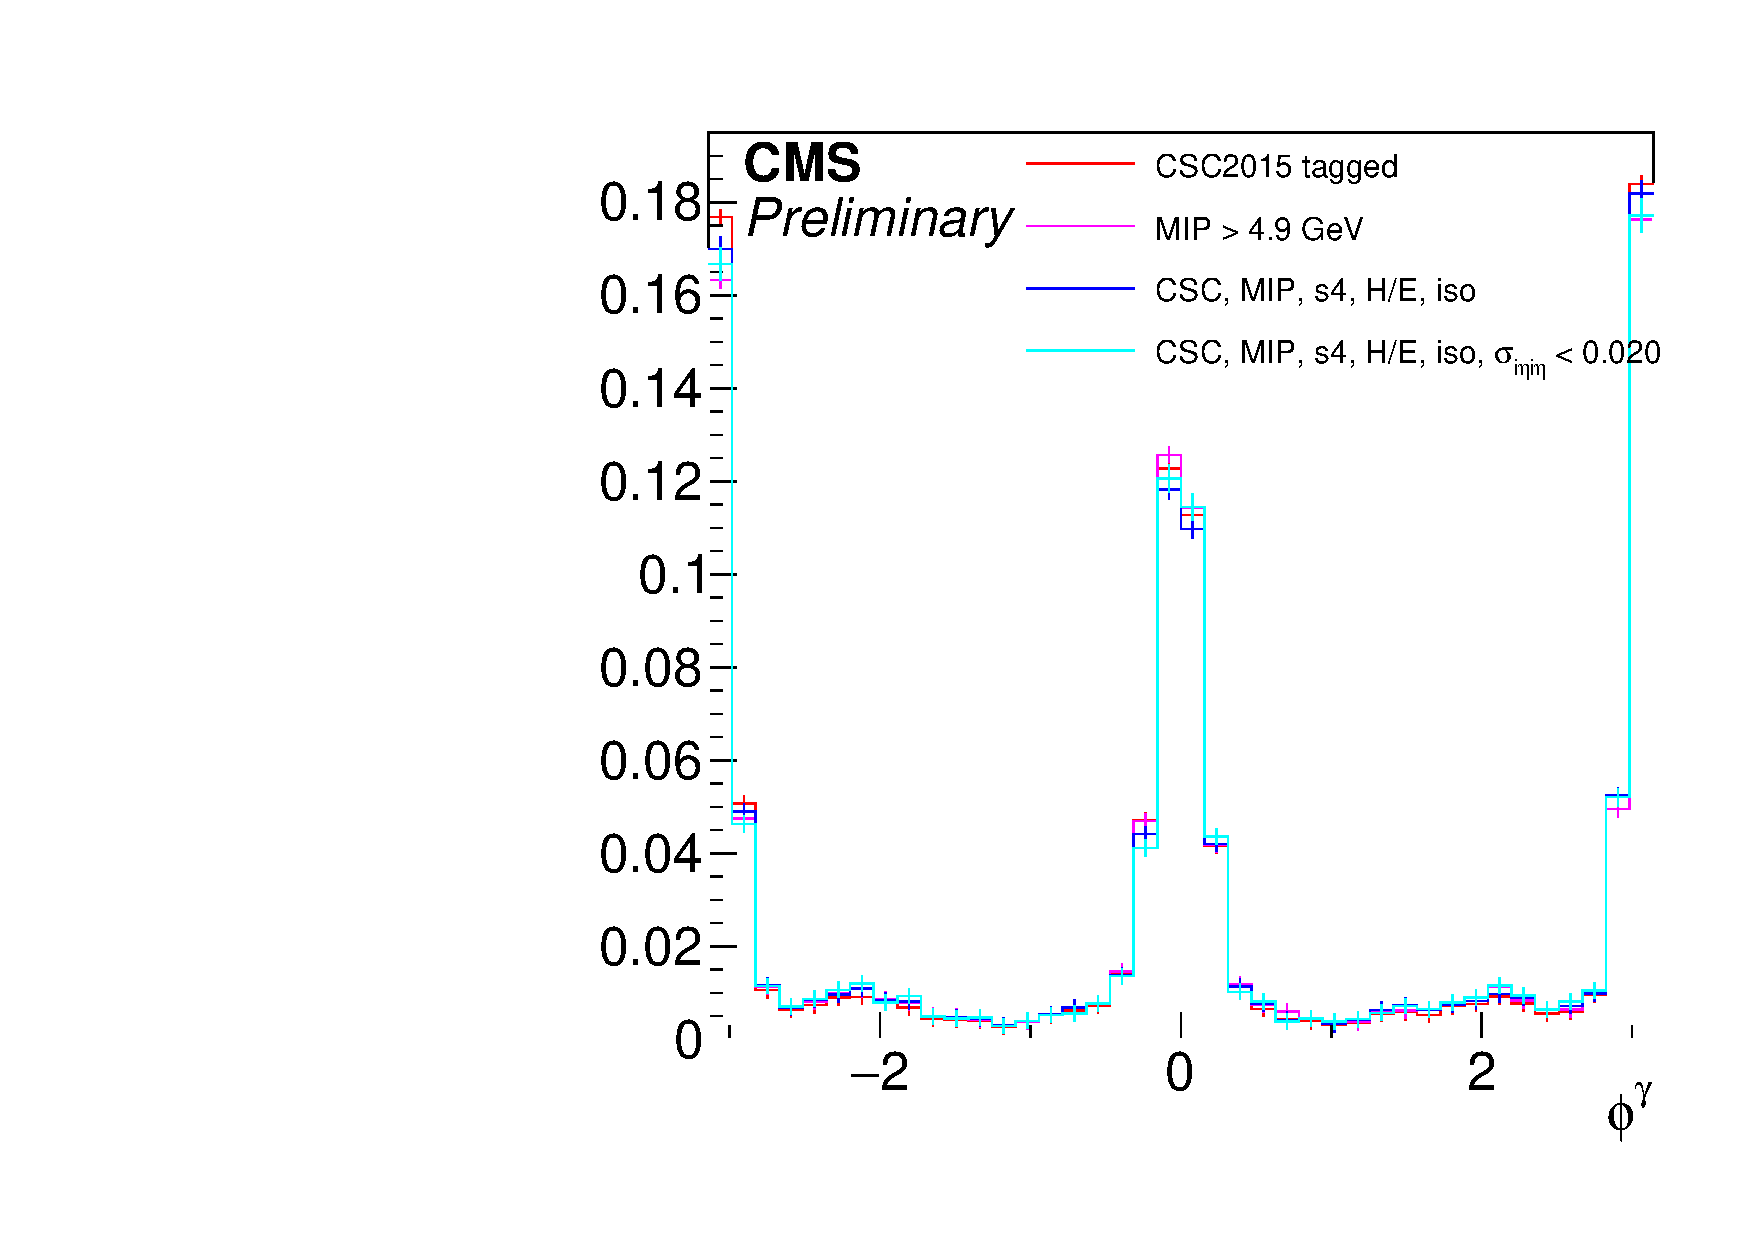
\includegraphics[width=0.6\textwidth]{Reconstruction/Figures/halo/halophi.pdf}
    \caption{
      The \phig\ distribution of the halo-like showers, tagged in multiple ways. 
      Histograms are normalized to unity.
      The cyan histogram is the \phig\ distribution after applying photon identification selections except for the shower shape. 
      It can be seen that the \phig\ distribution is highly stable against the listed identification selections.
    }
    \label{fig:halophi}
  \end{center}
\end{figure}

\begin{figure}[tbp]
  \begin{center}
    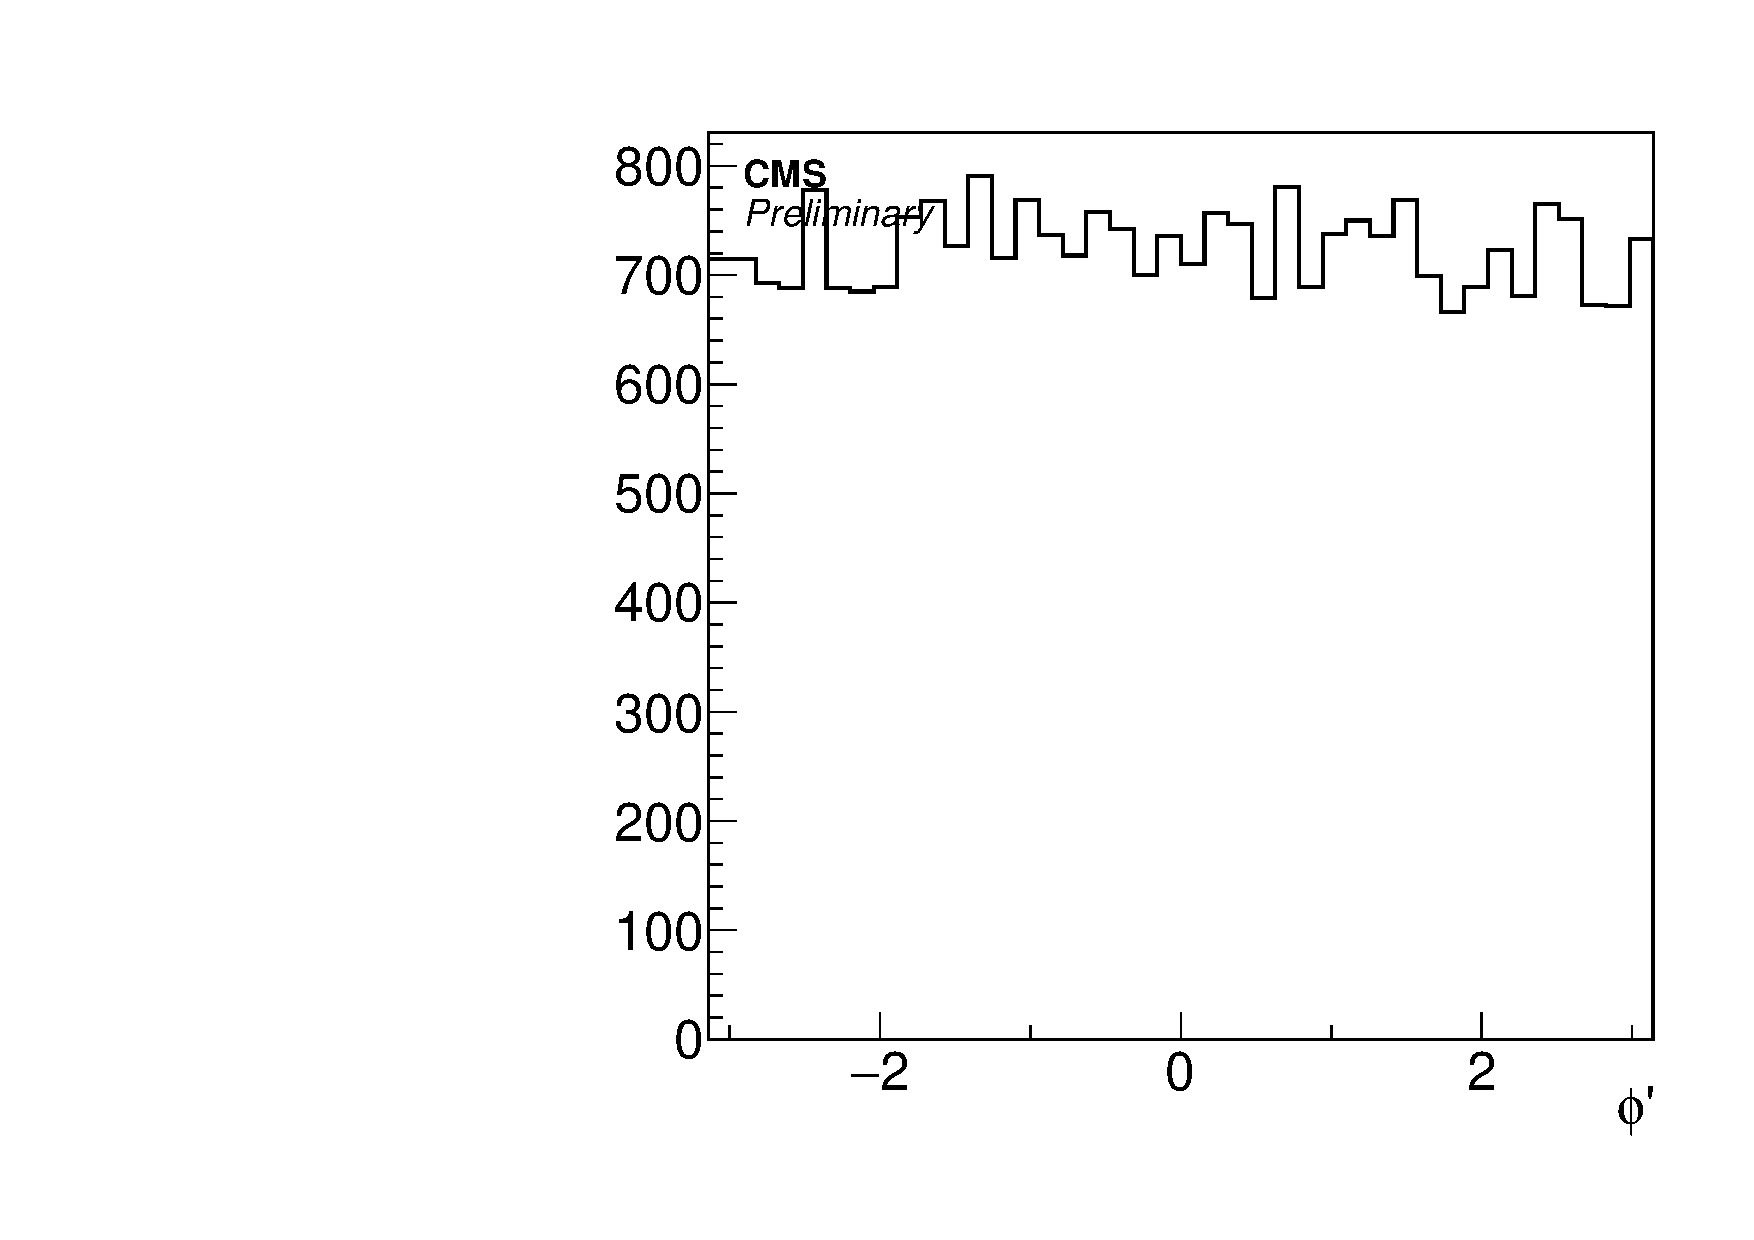
\includegraphics[width=0.6\textwidth]{Reconstruction/Figures/halo/bkgphi.pdf}
    \caption{
      The \phig\ distribution from \zinvg\ MC simulation.
    }
    \label{fig:bkgphi}
  \end{center}
\end{figure}

Because beam halo particles are produced through complex LHC machine effects, it is natural that the observed distribution of the halo showers is not
symmetric in the azimuthal angle in the detector coordinates.
Figure~\ref{fig:halophi} is a \phig\ distribution of the halo showers obtained from the Single Photon data set, requiring $\met > 140\GeV$. 
Here, halo showers are defined as those that fail the MIP-tagging and in the event tagged by the CSC beam halo tagger. 
On the other hand reconstructed shower from all other sources are symmetric in \phig\, as demonstrated in Fig.~\ref{fig:bkgphi}. 

\begin{figure}[tbp]
  \begin{center}
    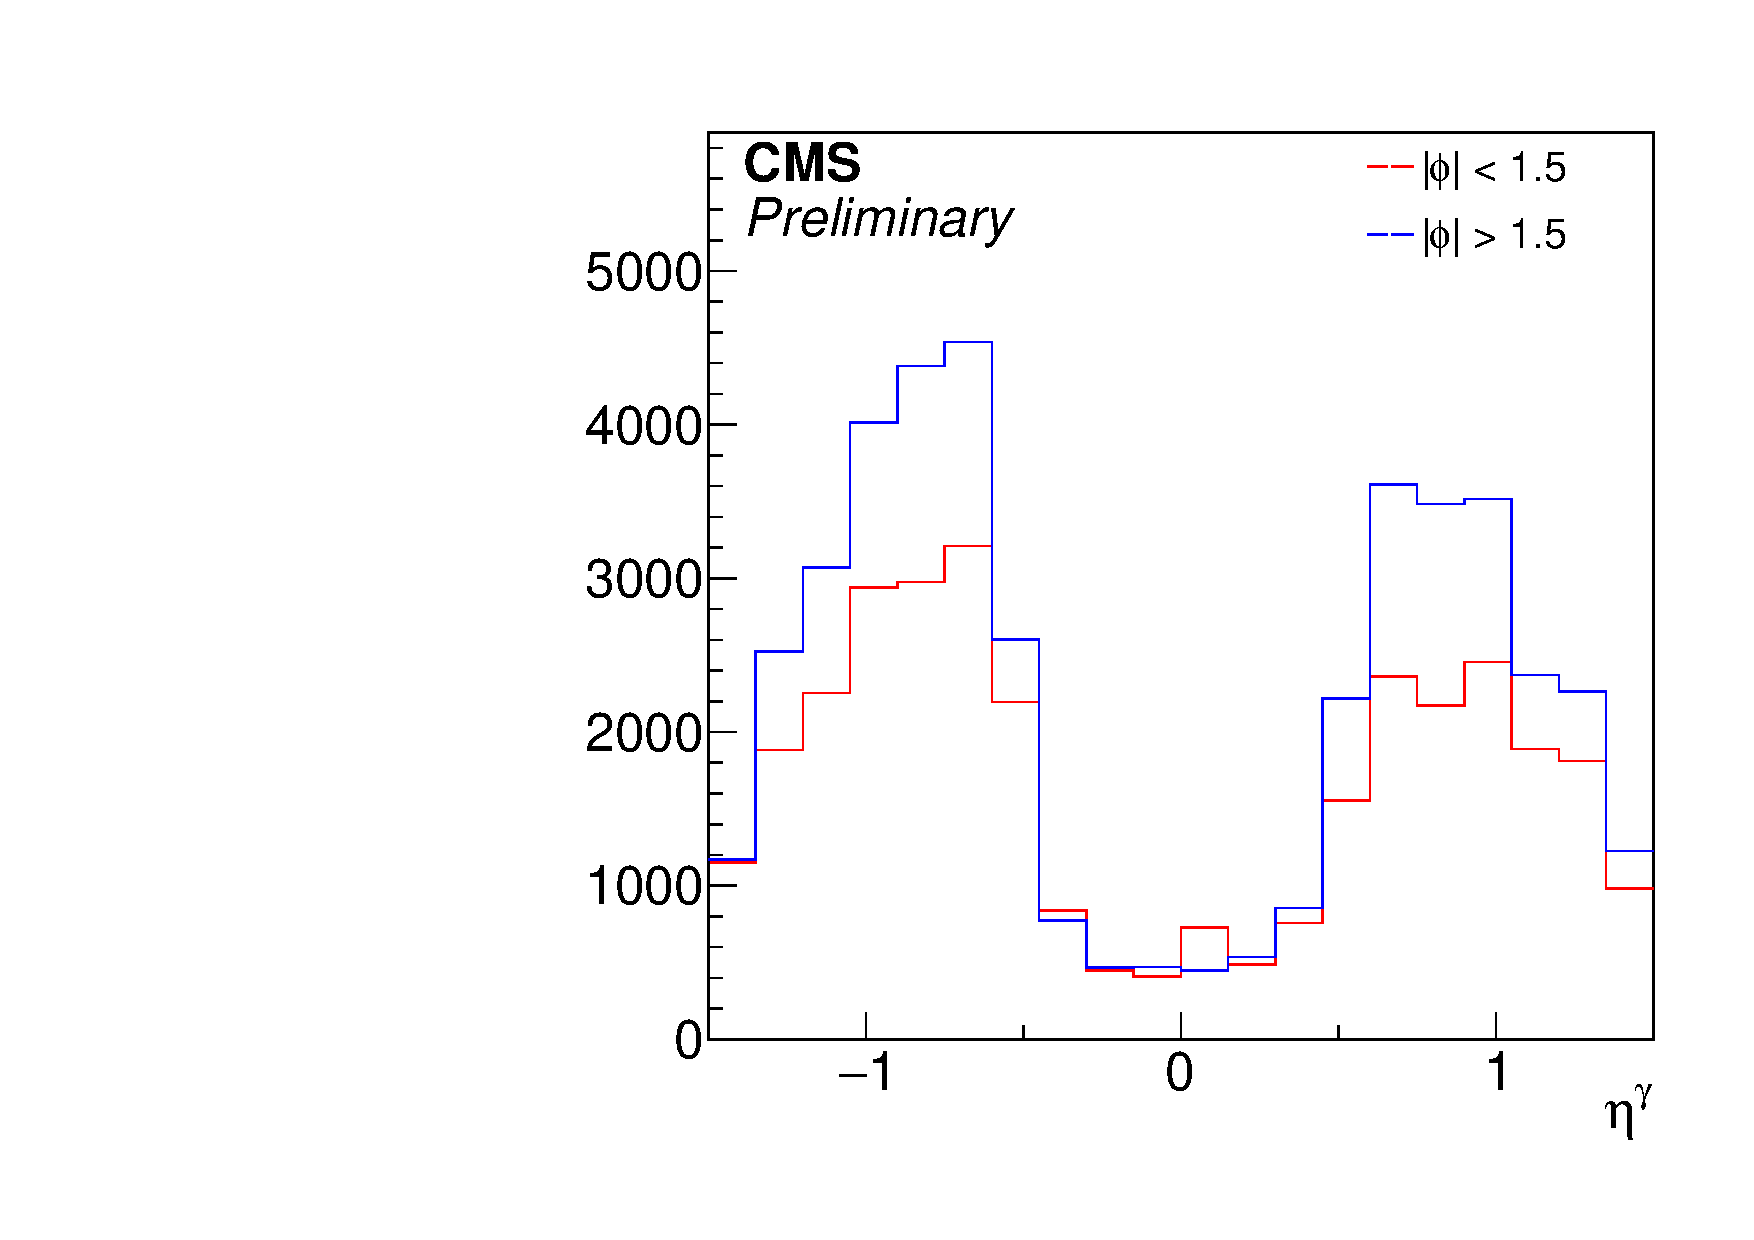
\includegraphics[width=0.7\textwidth]{Reconstruction/Figures/halo/halo_eta.pdf}
    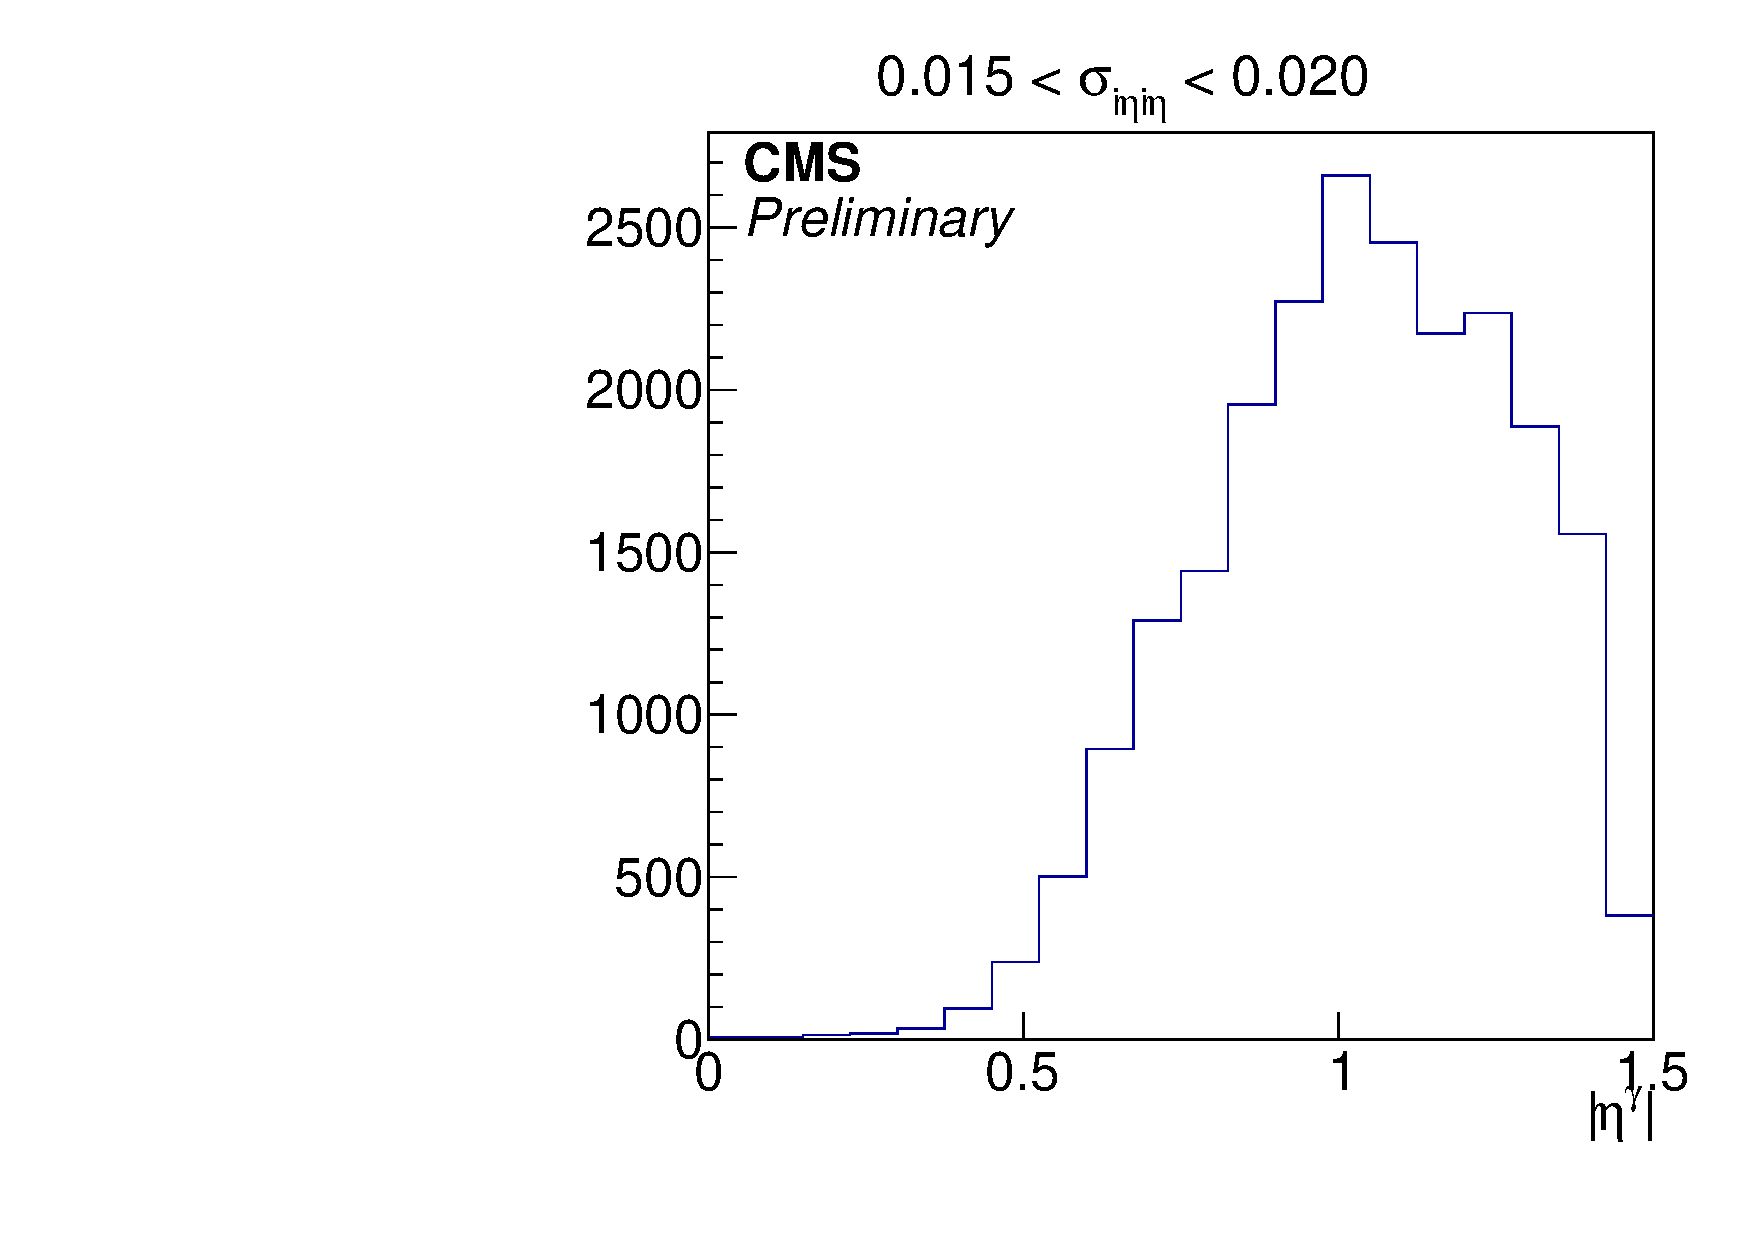
\includegraphics[width=0.45\textwidth]{Reconstruction/Figures/halo/halo_shape_etalow.pdf}
    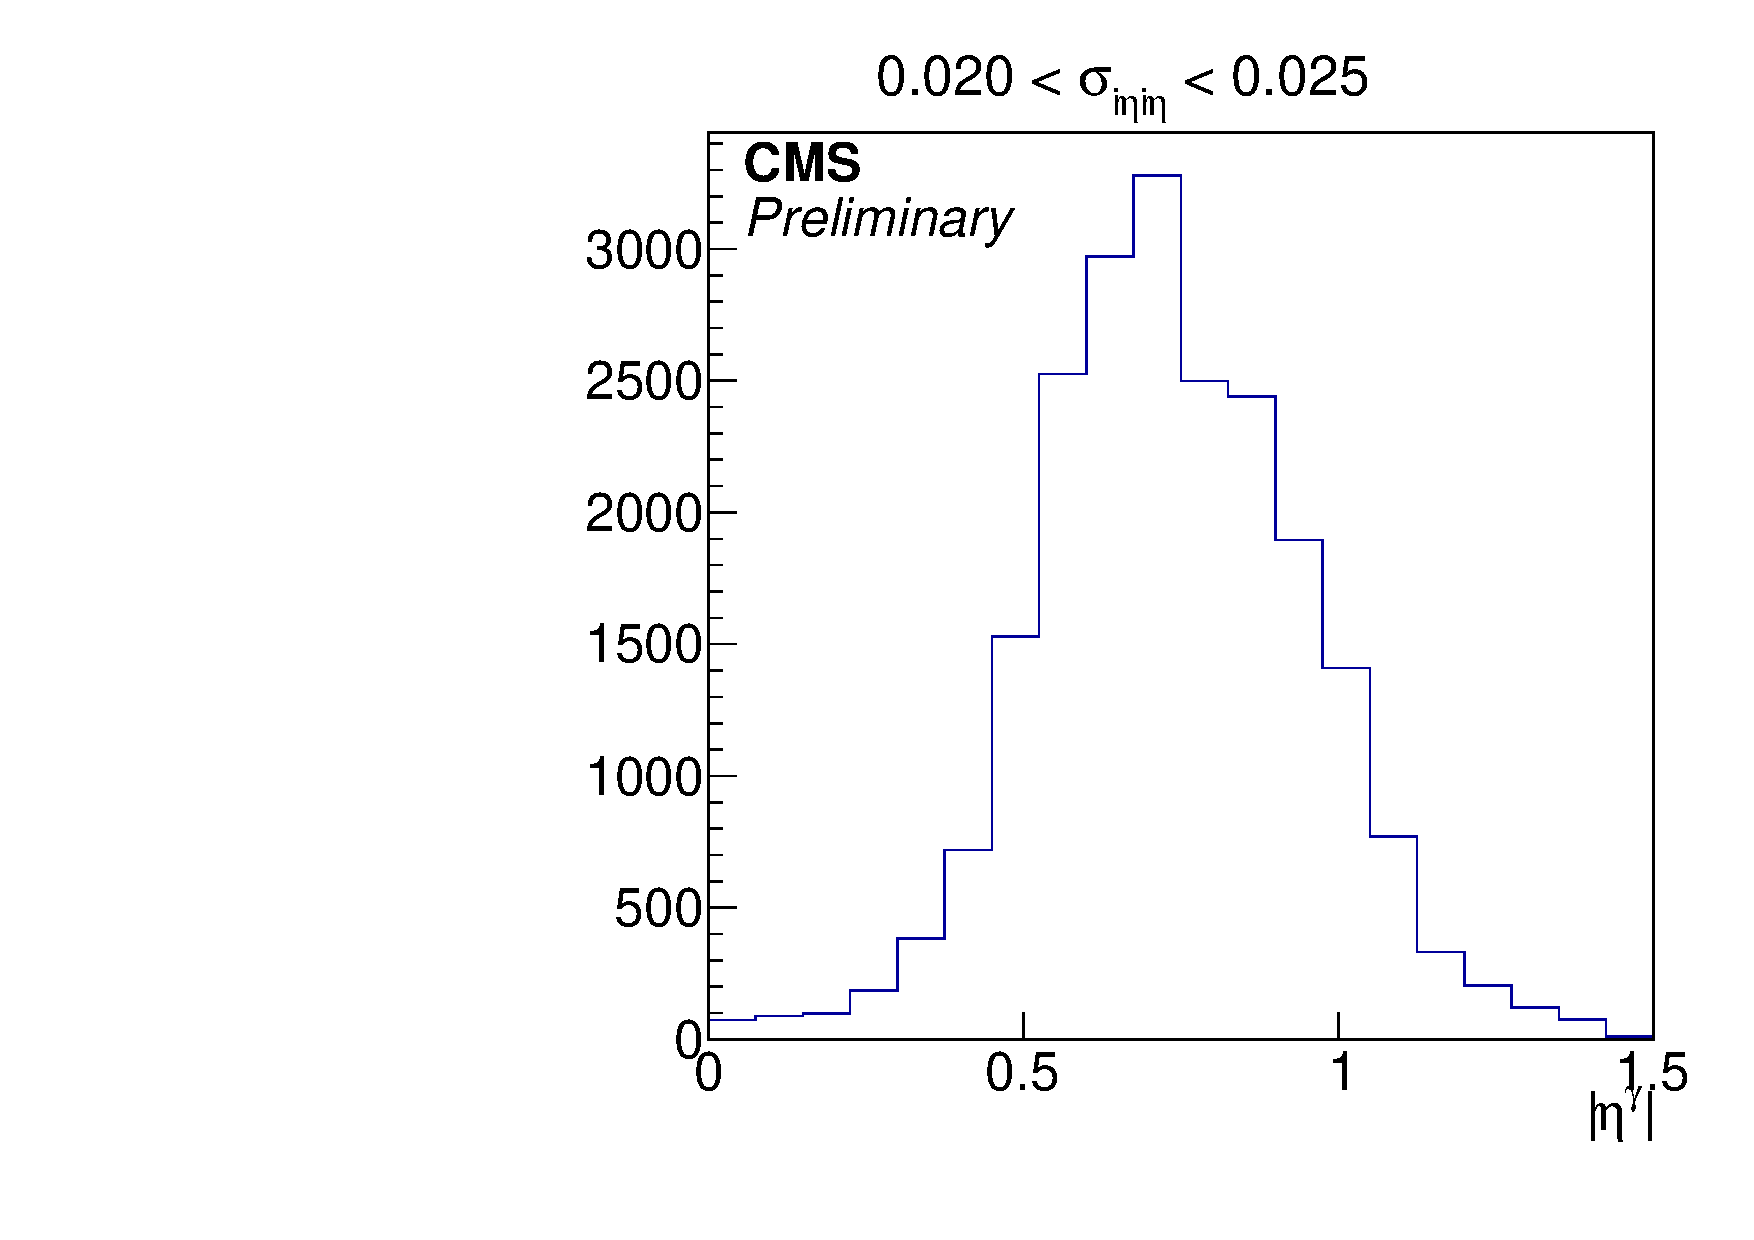
\includegraphics[width=0.45\textwidth]{Reconstruction/Figures/halo/halo_shape_etahigh.pdf}
    \caption{
      Top: $\eta$ distribution of the halo-like showers with $|\phi| < \pi/2$ and $|\phi| > \pi/2$.
      Bottom: shift in the $\eta$ distribution of the halo-like showers with respect to the requirement on \sieie.
    }
    \label{fig:halo_eta}
  \end{center}
\end{figure}

For the distribution of Fig.~\ref{fig:halophi} to be a valid template for halo showers, it must be first confirmed that its shape is invariant under photon selection requirements. 
However, further study of the \phig\ distribution of the halo showers indicates that the relative strength of the two prominent peaks in the distribution may change under the \sieie\ selection requirement.  
To explain this phenomenon, one needs to look at the the \etag\ distribution of the shower populations near $\phig \sim 0$ and $\phig \sim \pi$, shown in the top portion of Figure~\ref{fig:halo_eta}. 
Meanwhile, halo showers tend to have narrower shape in the $\eta$ direction when occurring at high $\eta$, due to the projective geometry of the ECAL crystals, visible in the bottom portion of Figure~\ref{fig:halo_eta} bottom). 
Combining the two observations, the conclusion is that the stringent requirement on the narrowness of the shower in the photon selection will preferentially reduce the $\phi \sim 0$ population.

\begin{figure}[tbp]
  \begin{center}
    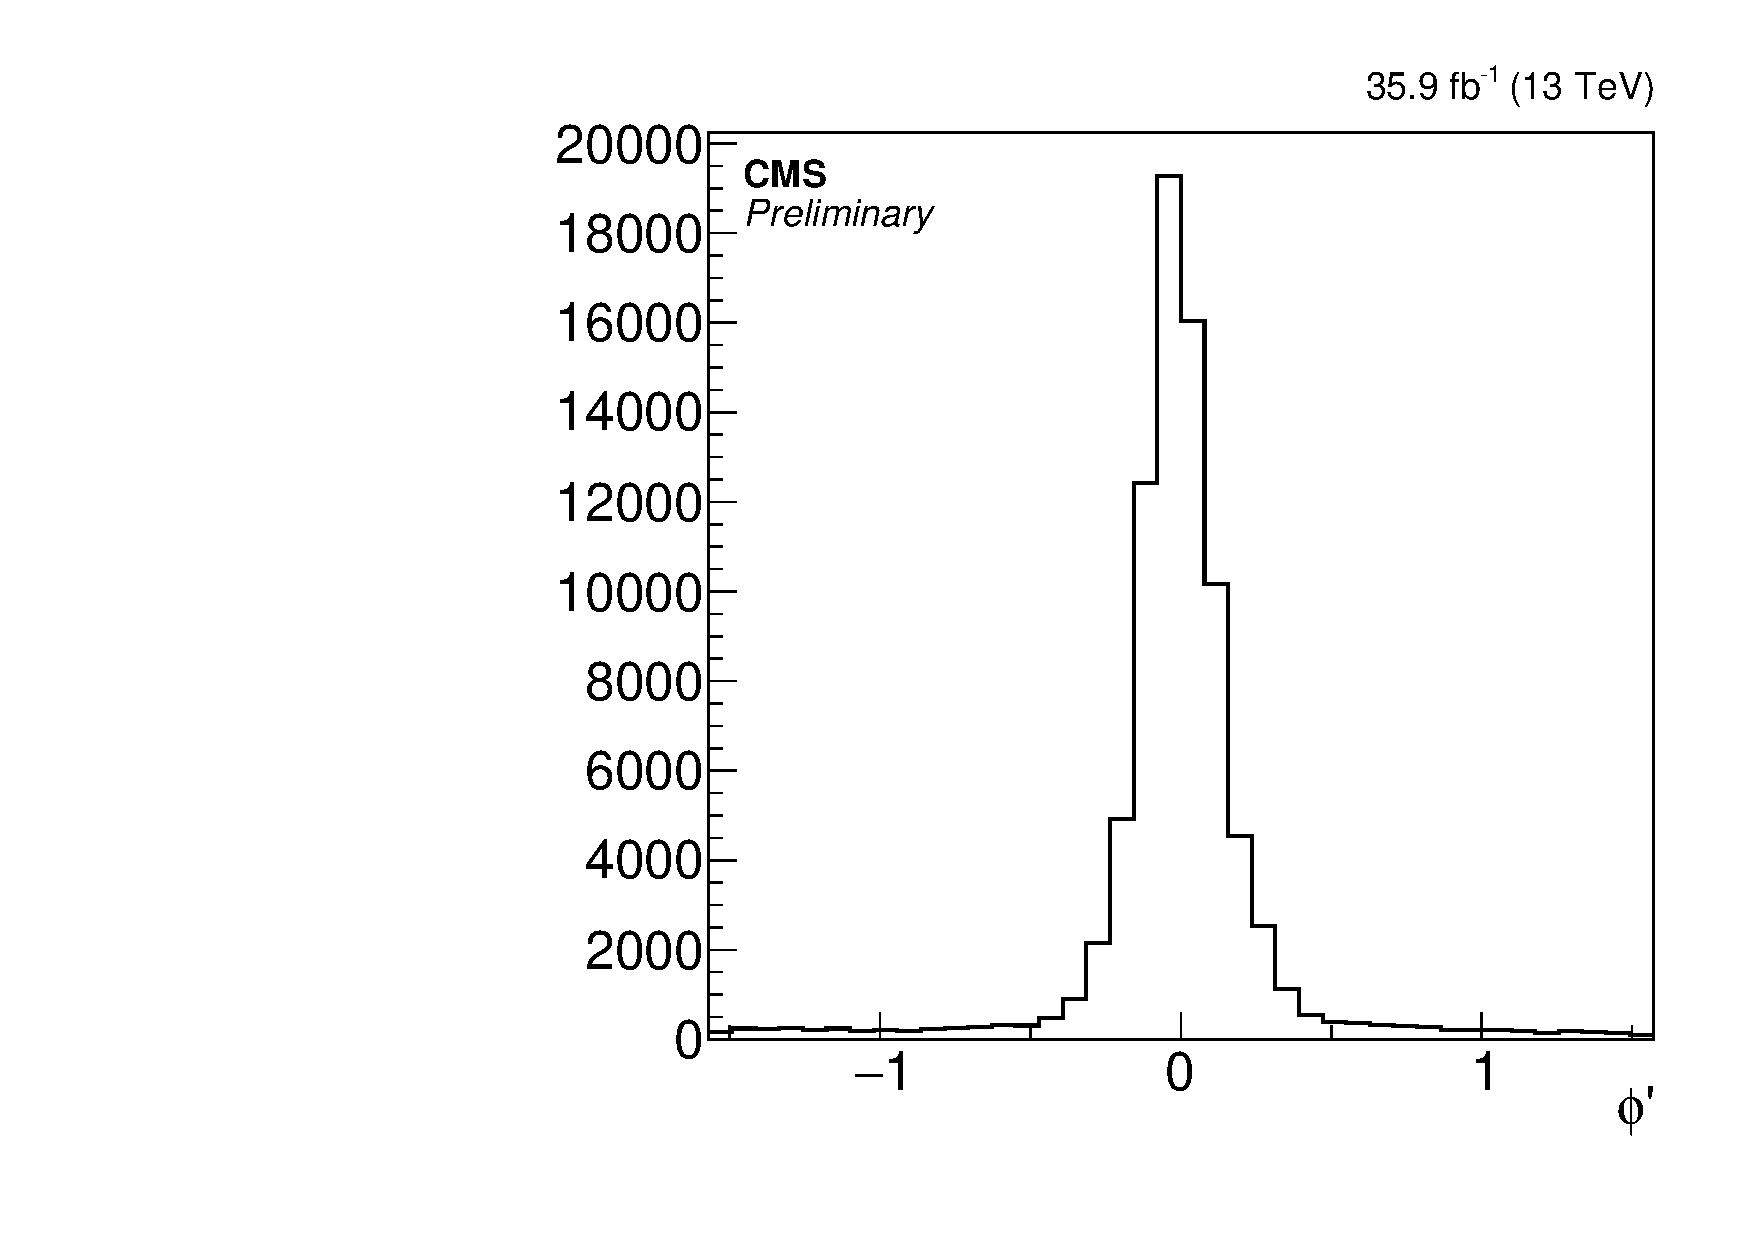
\includegraphics[width=0.45\textwidth]{Reconstruction/Figures/halo/haloPhiFolded.pdf}
    \caption{
      Folded $\phi'$ distribution of the halo sample.
    }
    \label{fig:halo_template}
  \end{center}
\end{figure}

Nevertheless, the invariance under photon selection is recovered by folding the \phig\ distribution such that the two peaks of the halo showers coincide.
To match the positions of the peaks in the halo template, the distribution is shifted by 0.005 and then folded along 0. 
The new angular variable $\phi'$
\begin{equation}
  \phi' := \left|\left[\left[\phig + 0.005\right]_{-\pi}^{\pi} - \frac{\pi}{2}\right]_{-\pi}^{\pi}\right| - \frac{\pi}{2},
\end{equation}
where $[\cdot]_{\pi}^{\pi}$ signifies casting the content into range $[-\pi,\pi]$,
exhibits a unimodal distribution for the halo template, as shown in Fig.~\ref{fig:halo_template}.

\begin{figure}[tbp]
  \begin{center}
    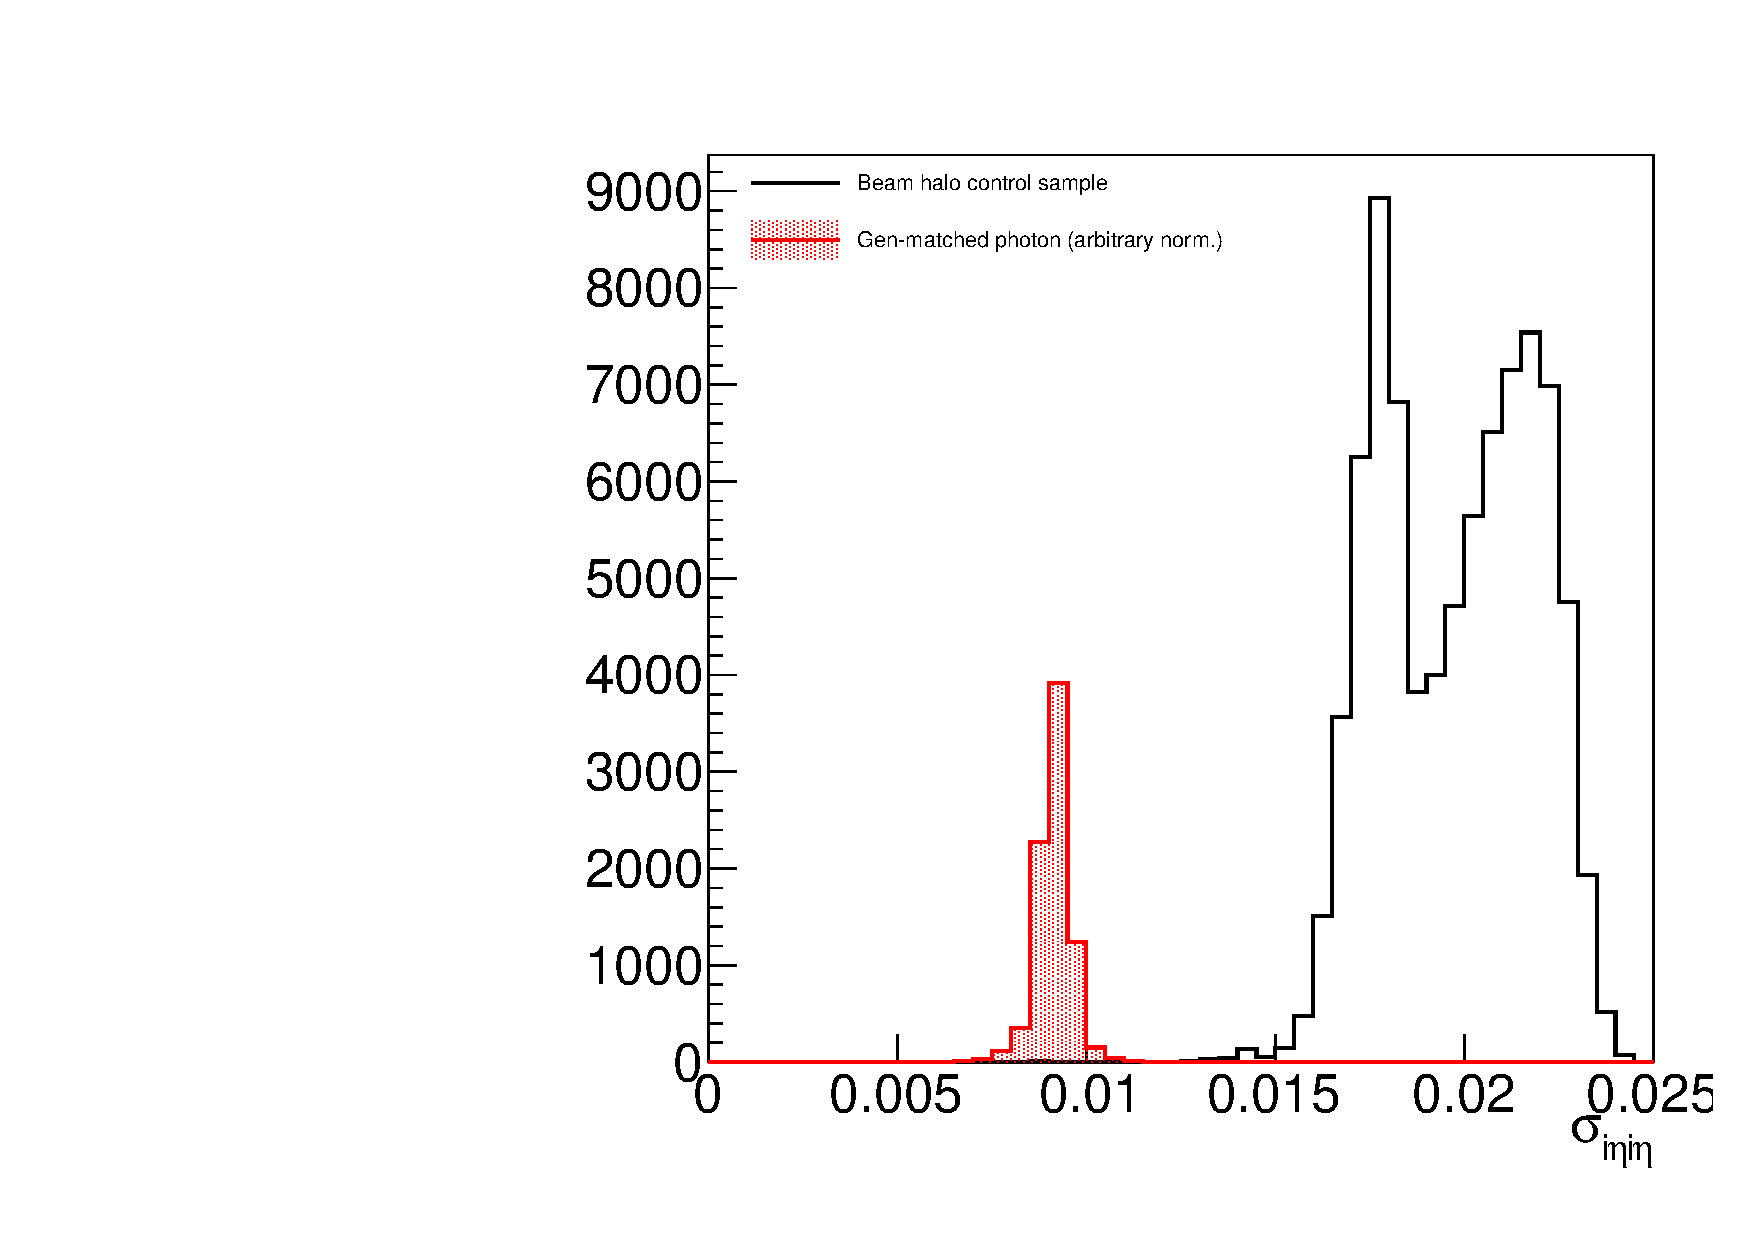
\includegraphics[width=0.45\textwidth]{Reconstruction/Figures/halo/halo_sieie.pdf}
    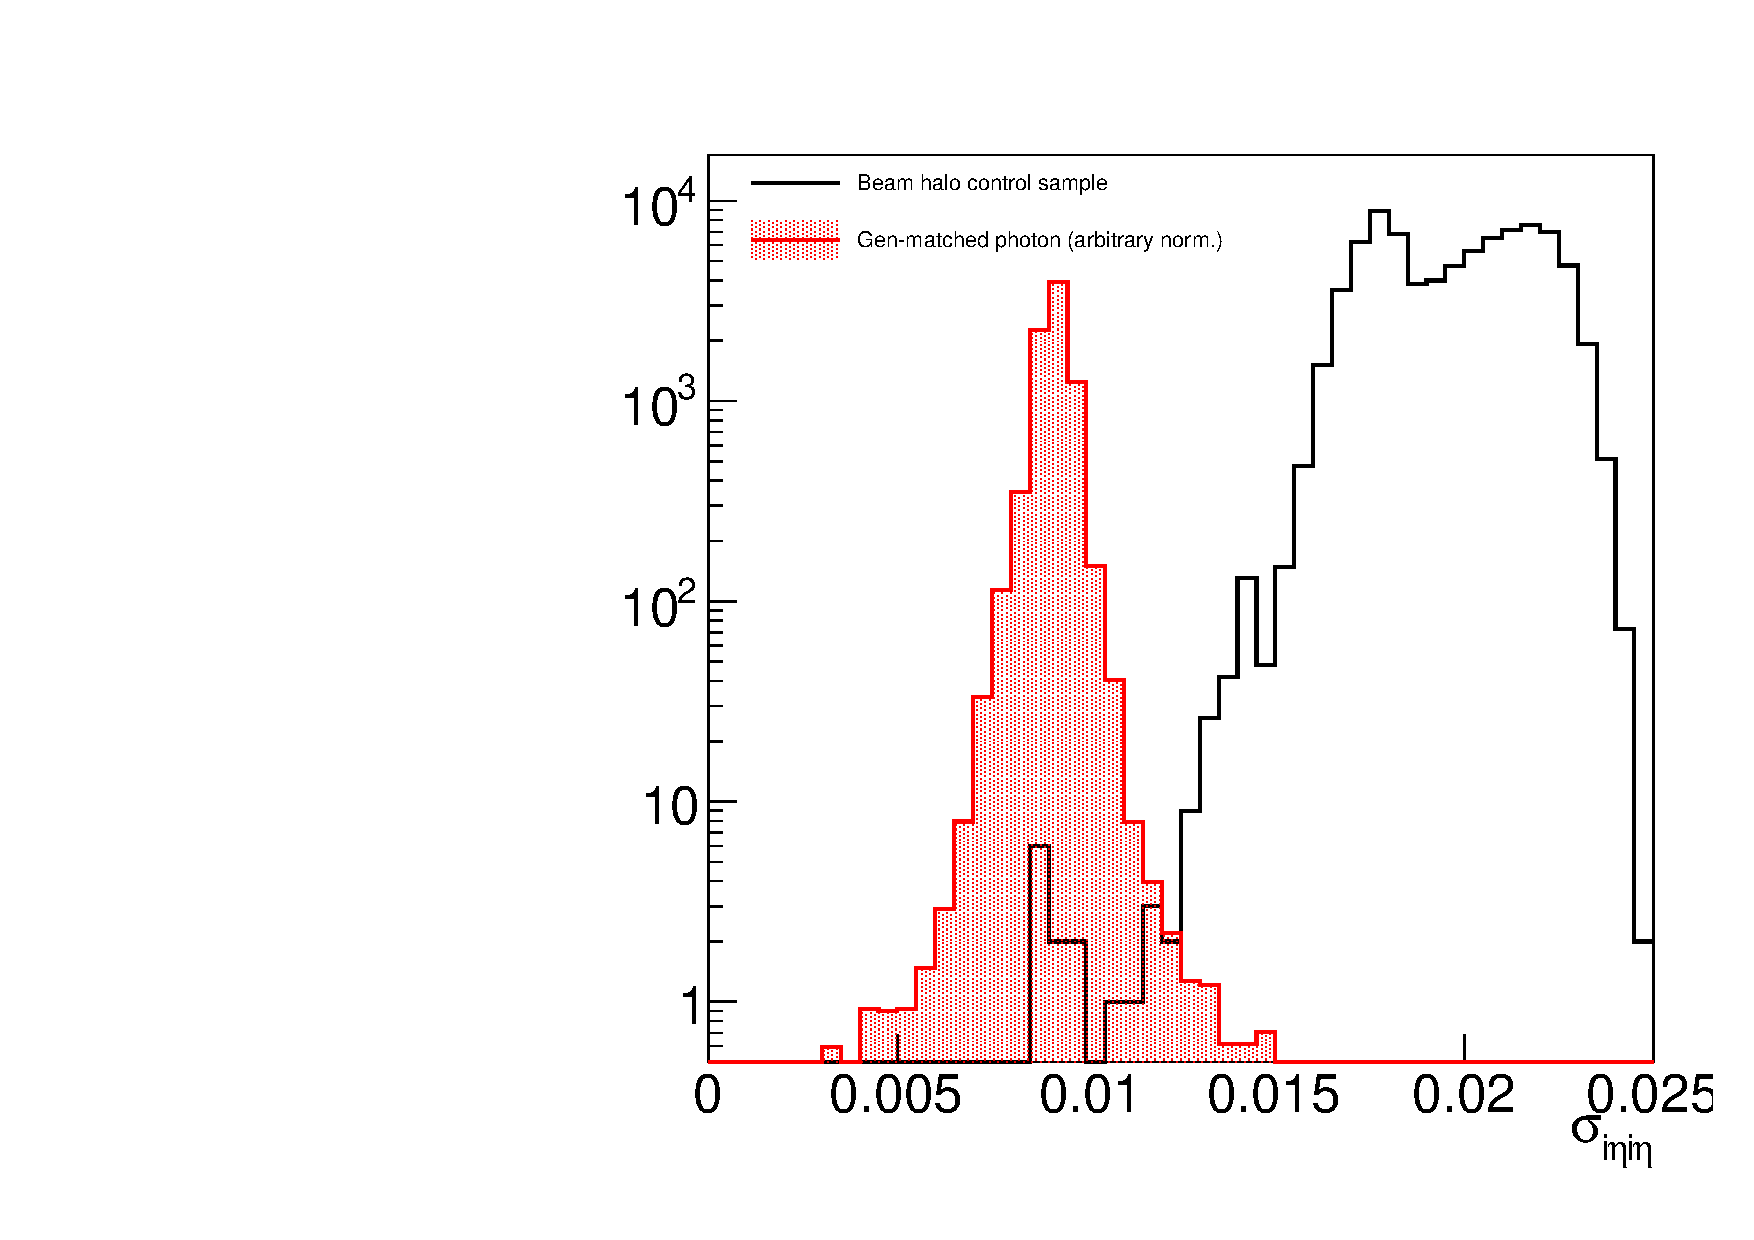
\includegraphics[width=0.45\textwidth]{Reconstruction/Figures/halo/halo_sieie_log.pdf}
    \caption{
      The \sieie distribution of the beam halo control sample and a reference distribution from truth-matched MC photons. 
      Left: linear scale, Right: log scale. 
      There is a small peak at $\sieie \sim 0.01$ in the beam halo control sample, which is not visible in linear-scale.
    }
    \label{fig:halo_sieie}
  \end{center}
\end{figure}

The contribution of real photons into the halo control sample is negligible.
This is confirmed from the \sieie\ distribution of the halo control sample and the correlation between \sieie\ and \emip\ in a MC true-photon sample.
The \sieie\ distribution of the halo control sample features a small peak at $\sieie \sim 0.01$, which can be attributed to contributions from true photons, as the photon \sieie distribution overlaid in Figure~\ref{fig:halo_sieie} suggests. 
However, the contribution of true photons diminishes rapidly with increasing \sieie. 
Additionally, Figure~\ref{fig:sieie_mip_corr} illustrates that the shape of the true-photon \sieie does not change significantly with respect to \emip. 
From these two observations, we can see that there are is only a negligible number of true photons in the halo control sample.

\begin{figure}[tbp]
  \begin{center}
    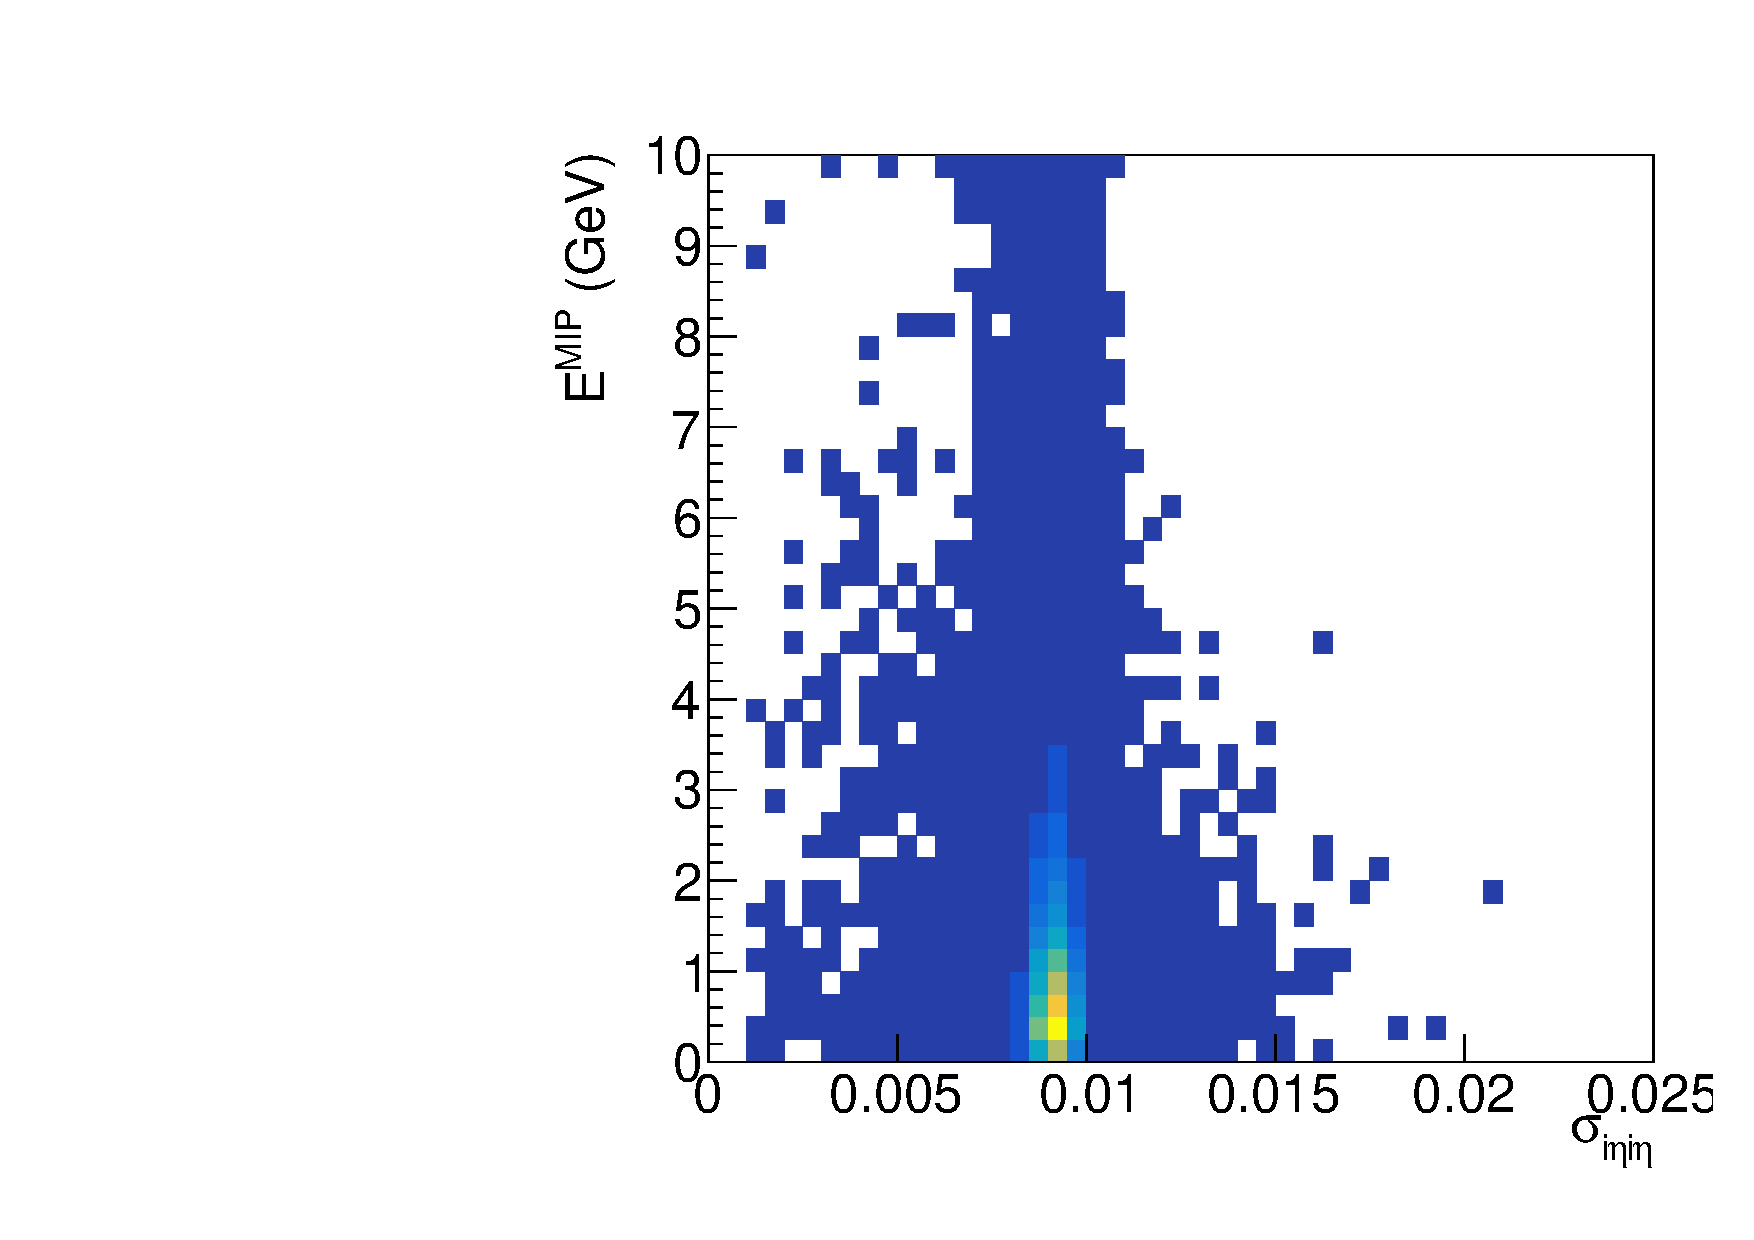
\includegraphics[width=0.45\textwidth]{Reconstruction/Figures/halo/sieie_mip_corr.pdf}
    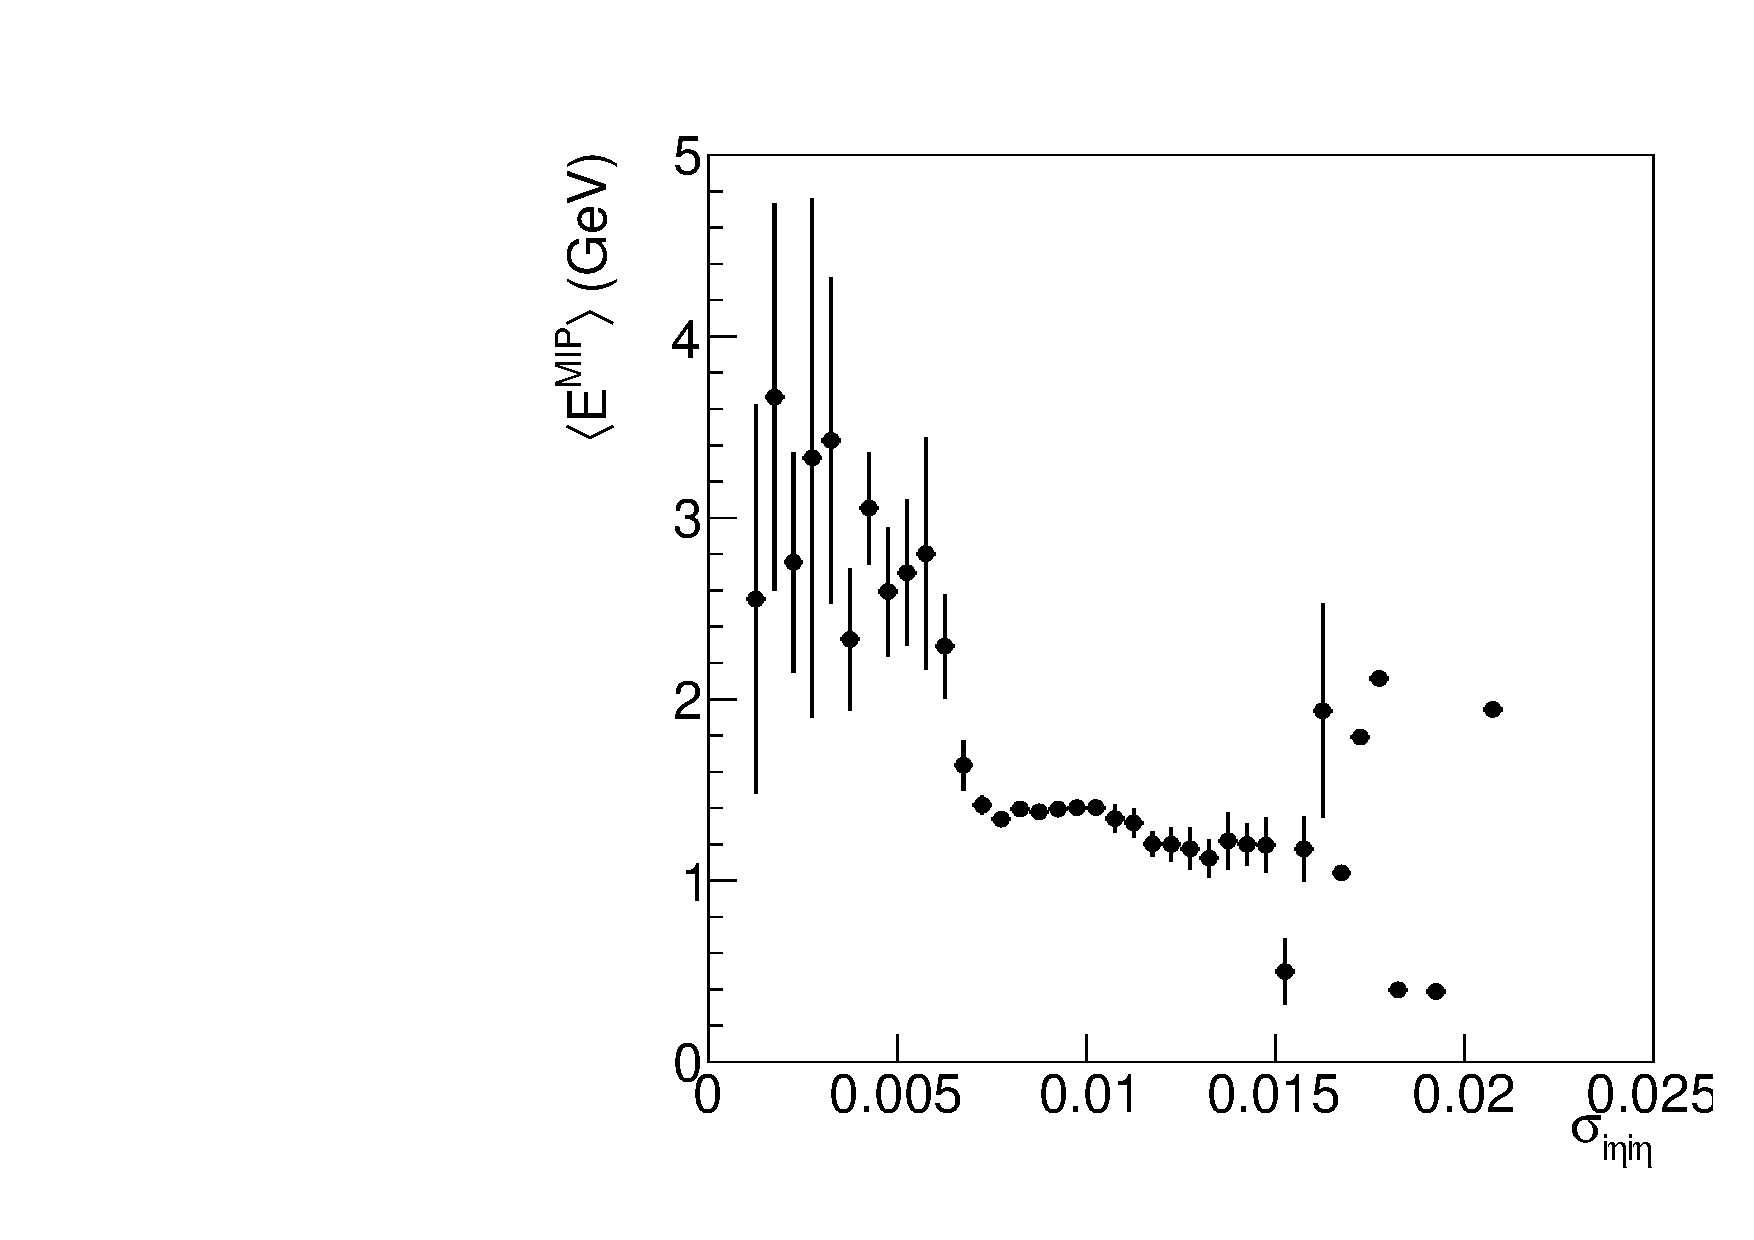
\includegraphics[width=0.45\textwidth]{Reconstruction/Figures/halo/sieie_mip_prof.pdf}
    \caption{
      Correlation between \sieie and \emip\ in truth-matched MC photons. 
      Left: \emip-\sieie distribution.
      Right: average \emip\ in bins of \sieie.
    }
    \label{fig:sieie_mip_corr}
  \end{center}
\end{figure}

While the peaking behavior is a robust feature of the halo showers, their rate is not easily predictable. 
Therefore, the contribution from beam halo processes is estimated by a direct fit to the observed data during the signal extraction process, described in Section~\ref{sec:halo_estimate}

\subsection{ECAL Barrel Spikes Phenomenology}
\label{sec:spikes}

Noise in the photodetector or the detector electronics can result in spurious photon signals. 
Most of the time, such spurious signal is filtered out by multiple layers of protection, starting from the so-called ``spike killer'' algorithm at the level-1 trigger~\cite{CMS_AN_2010-357}. 
Nevertheless, in rare cases, noise in a single ECAL channel coincides with pileup or other energy deposit in the nearby crystals and appear as a high-energy photon cluster.

\begin{figure}[tbp]
  \begin{center}
    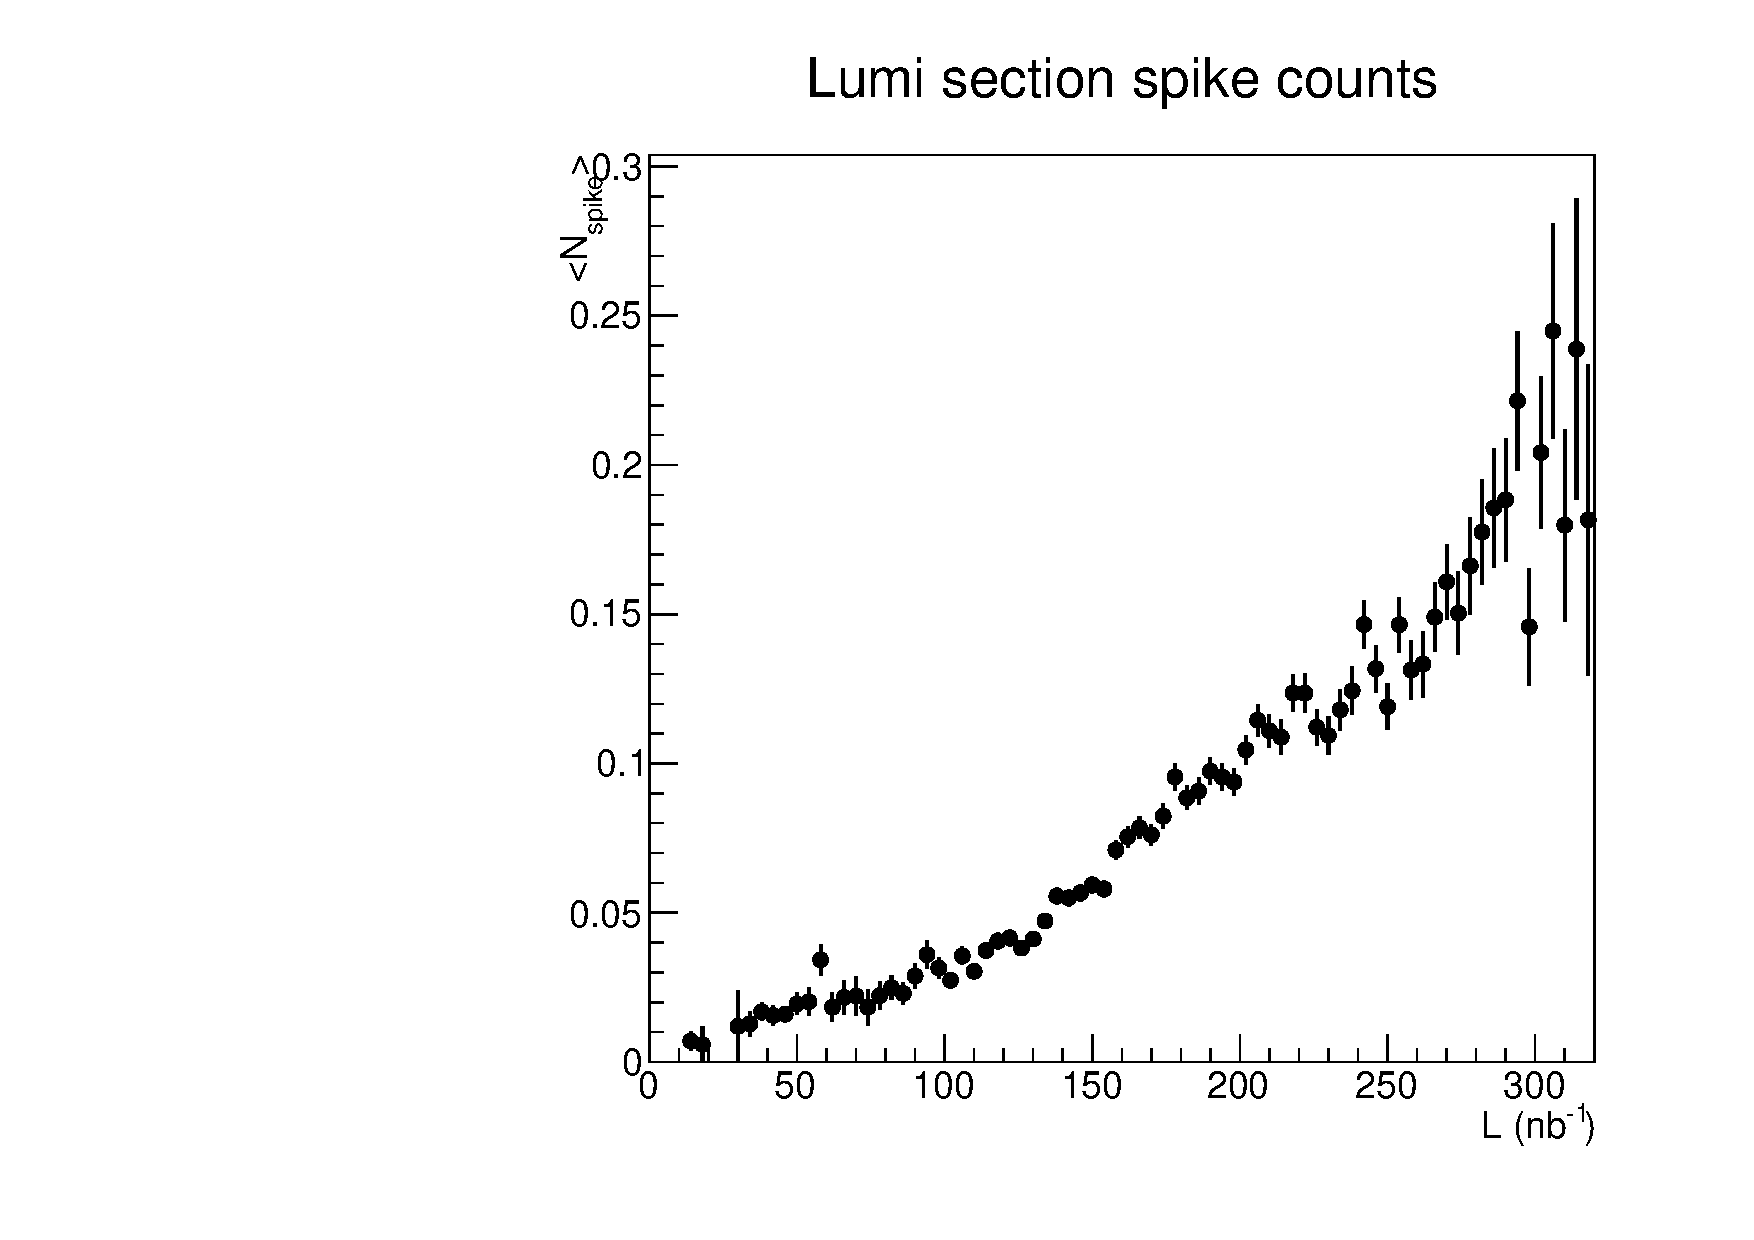
\includegraphics[width=0.45\textwidth]{Reconstruction/Figures/spikes/spike_lumi_scaling.pdf}
    \caption{
      Average number of spike clusters in a luminosity section, identified by $\sieie < 0.001$ and $E > 50\GeV$, in muon-triggered events, versus integrated luminosity of the luminosity section.
    }
    \label{fig:spike_lumi_scaling}
  \end{center}
\end{figure}

The origin of ECAL spikes is believed to be interactions of neutrons and other hadronic particles (collectively called neutral hadrons hereafter) with the photocathode material of the ECAL avalanche photo diodes (APD). 
Nuclear fission at the APD surface then causes a large electron avalanche, which is mistaken as a large photon yield scintillation in the ECAL crystal. 
Evidences supporting this hypothesis is documented in Ref.~\cite{CMS_AN_2010-357}. 
In Figure~\ref{fig:spike_lumi_scaling}, scaling of the rate of spikes with the instantaneous luminosity is confirmed, up to much higher luminosity values than was observed at the time when Ref.~\cite{CMS_AN_2010-357} was written.

A known feature of such spurious photon clusters is that the recorded pulse shape of the seed crystal, \ie, the channel with the noise, is not what is expected from a real electromagnetic shower in ECAL. 
In particular, this translates to a distinctive early rec hit time distribution, since the rec hit time is extracted from a fit to the pulse shape assuming a normal pulse.

In the normal CMS data reconstruction, rec hits that are tagged as spike-like are ignored in clustering. 
Rec hits are tagged as spikes if there is very little energy deposit recorded in the surrounding crystals, or if the reconstructed time is out of an allowed window.
Identical algorithms are employed in the HLT and offline reconstructions.

\begin{figure}[tbp]
  \begin{center}
    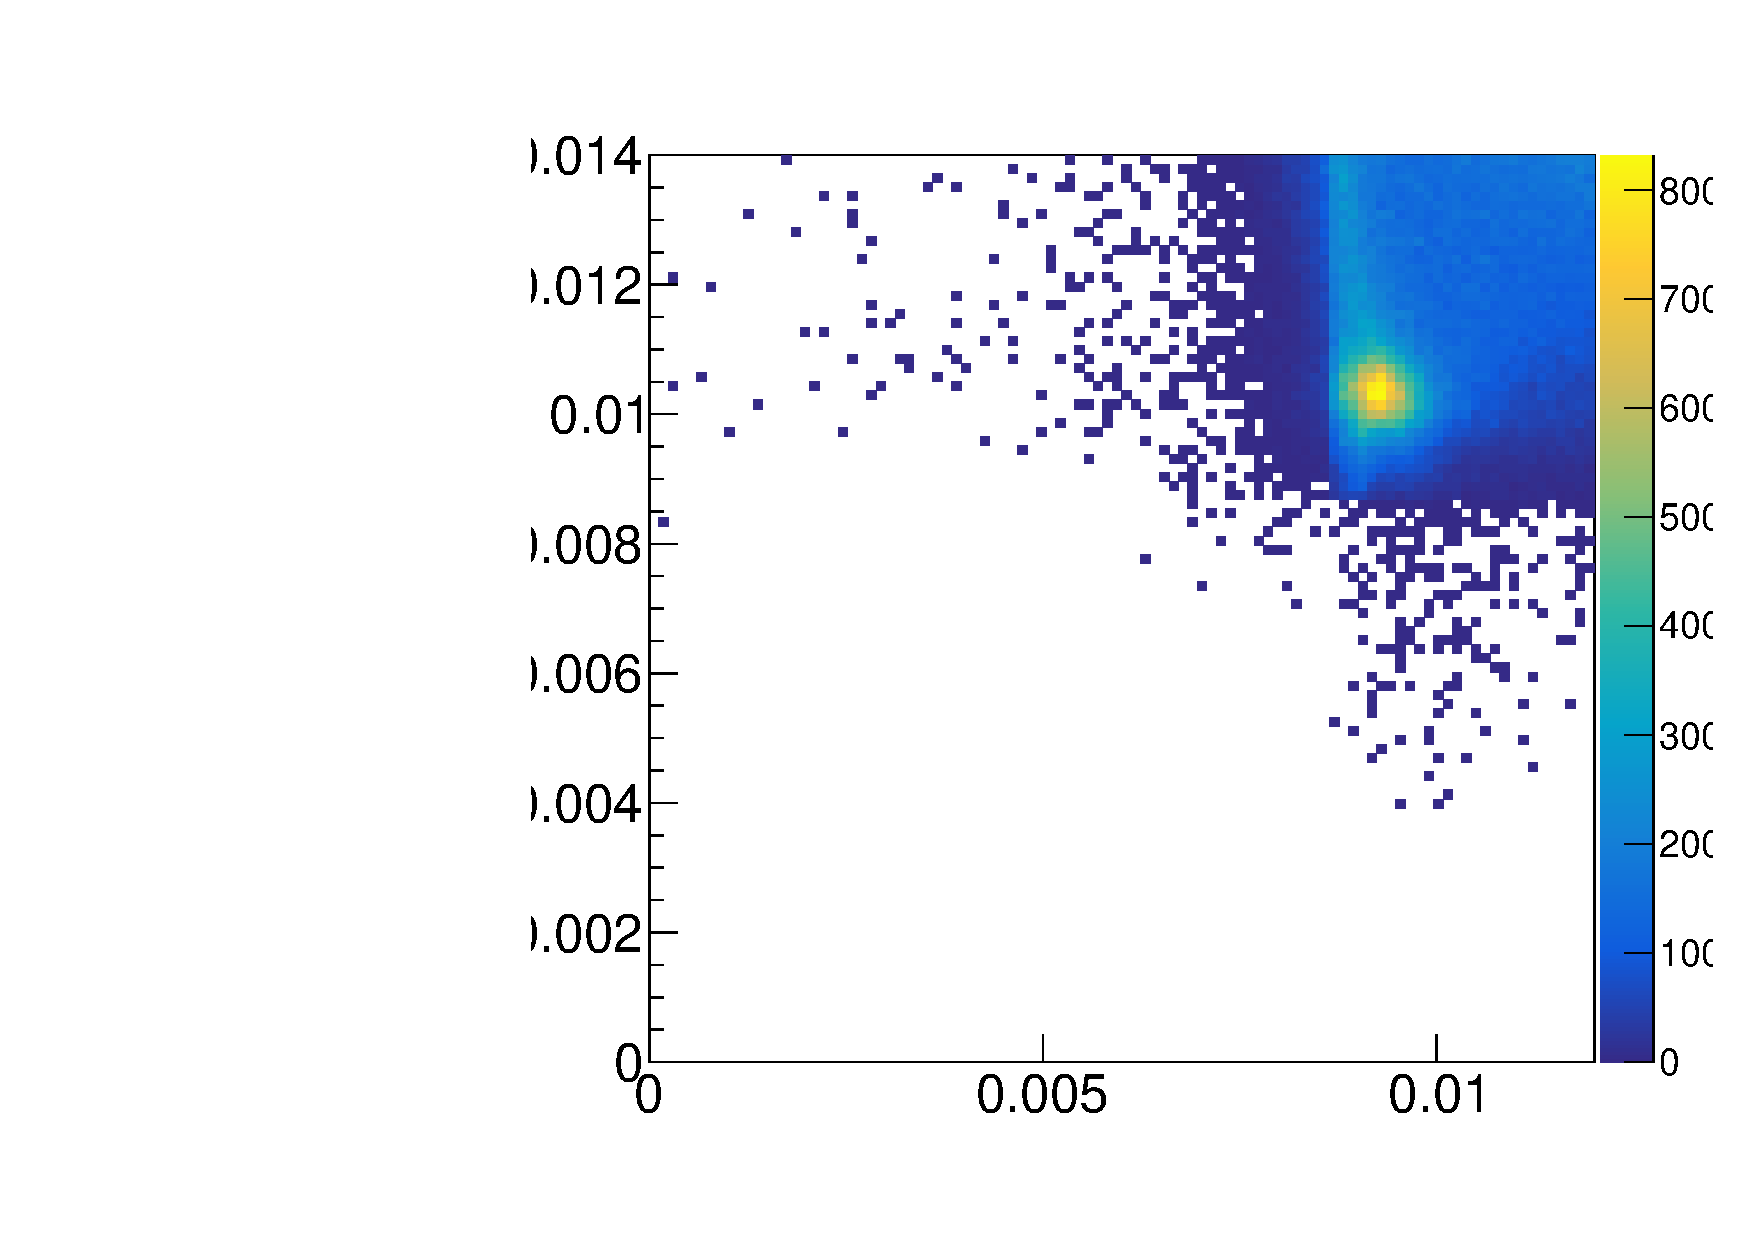
\includegraphics[width=0.45\textwidth]{Reconstruction/Figures/spikes/showershapes_standard.pdf}
    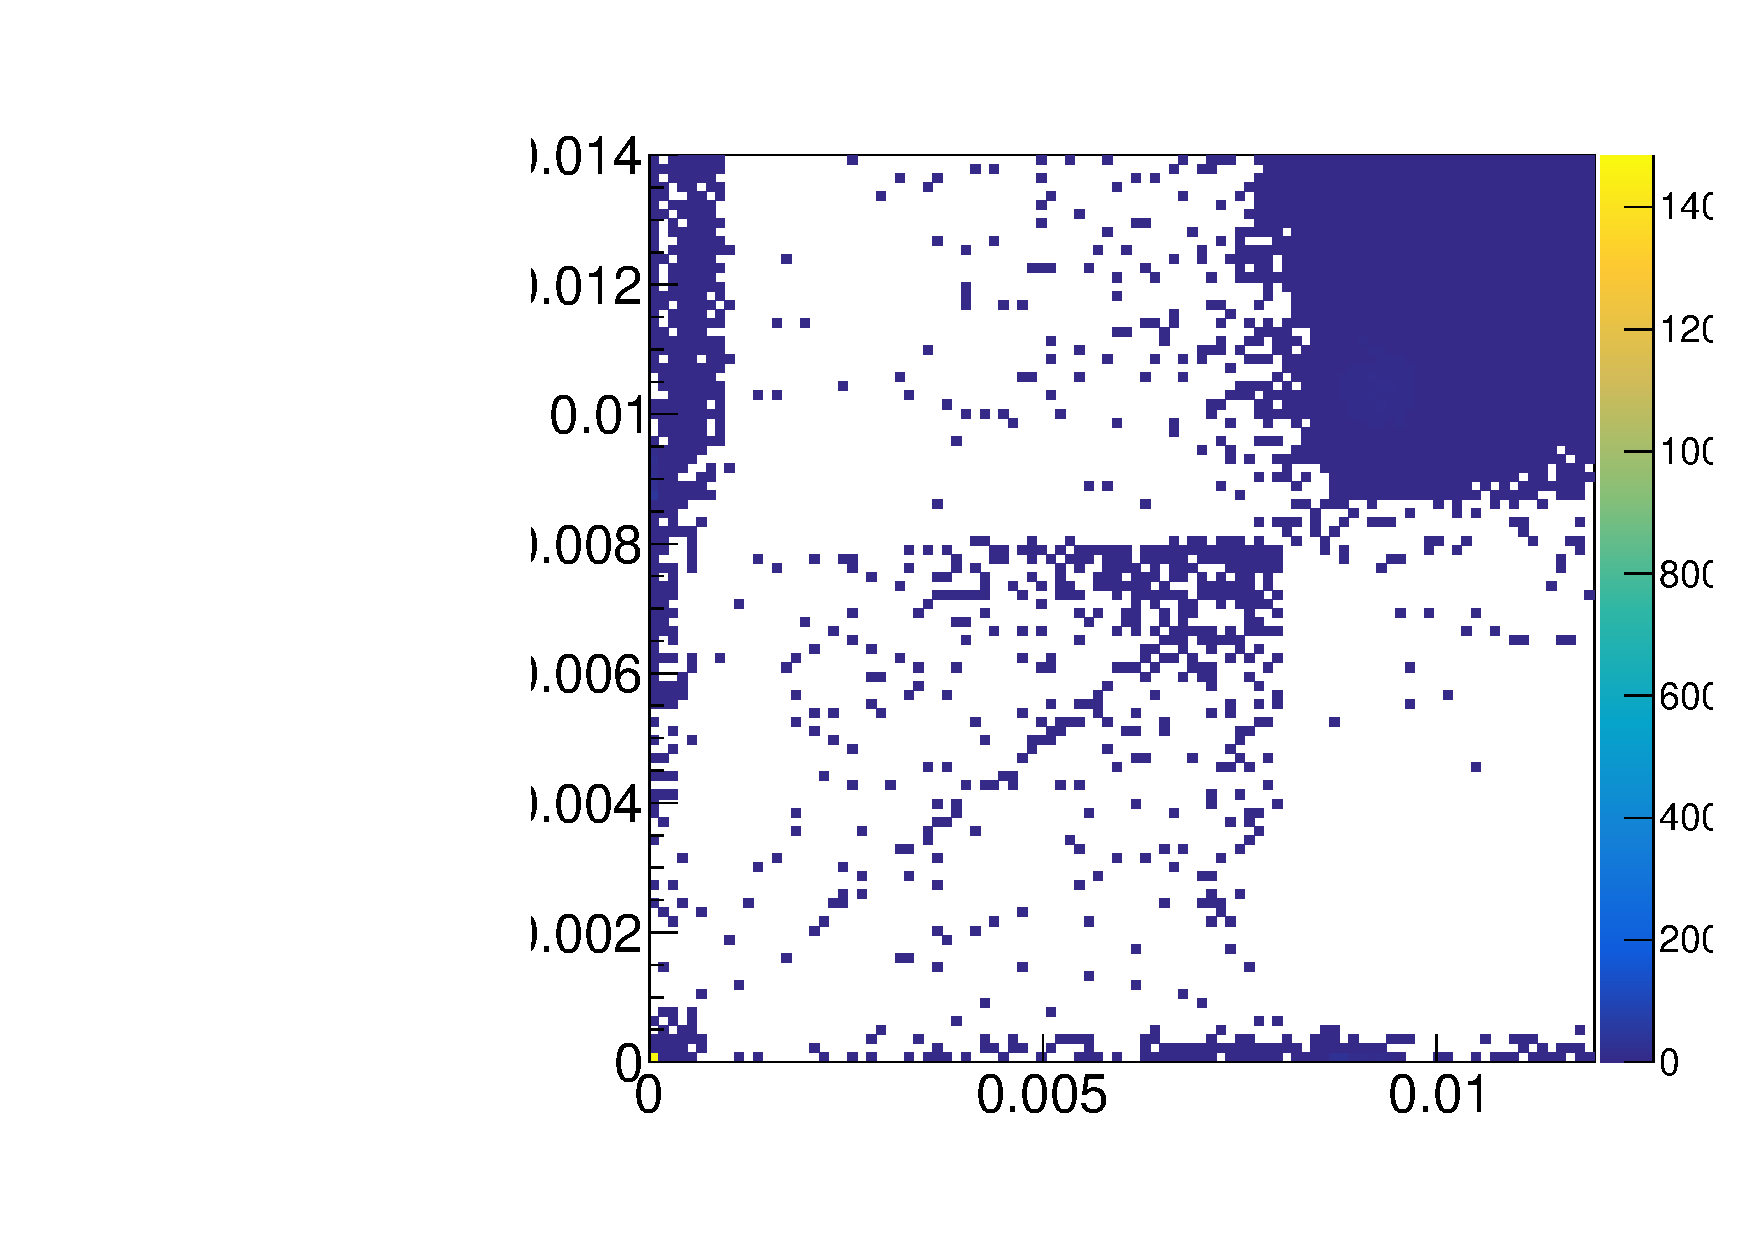
\includegraphics[width=0.45\textwidth]{Reconstruction/Figures/spikes/showershapes_uncleaned.pdf}
    \caption{
      Two-dimensional distributions in \sipip\ and \sieie\ of ECAL clusters in the standard reconstruction (left) and the special reconstruction with no spike cleaning (right).
    }
    \label{fig:showershape_map}
  \end{center}
\end{figure}

To study an unbiased spike sample, ECAL DIGI samples stored in the SingleMuon AOD datasets are reconstructed into ECAL clusters with no spike cleaning applied. 
DIGIs associated with the standard and ``uncleaned'' photon objects are stored in AOD, and ones for the uncleaned photons is rich in spike-like hits. 
Figure~\ref{fig:showershape_map} shows how narrow clusters are cleaned away in the normal reconstruction.

\begin{figure}[tbp]
  \begin{center}
    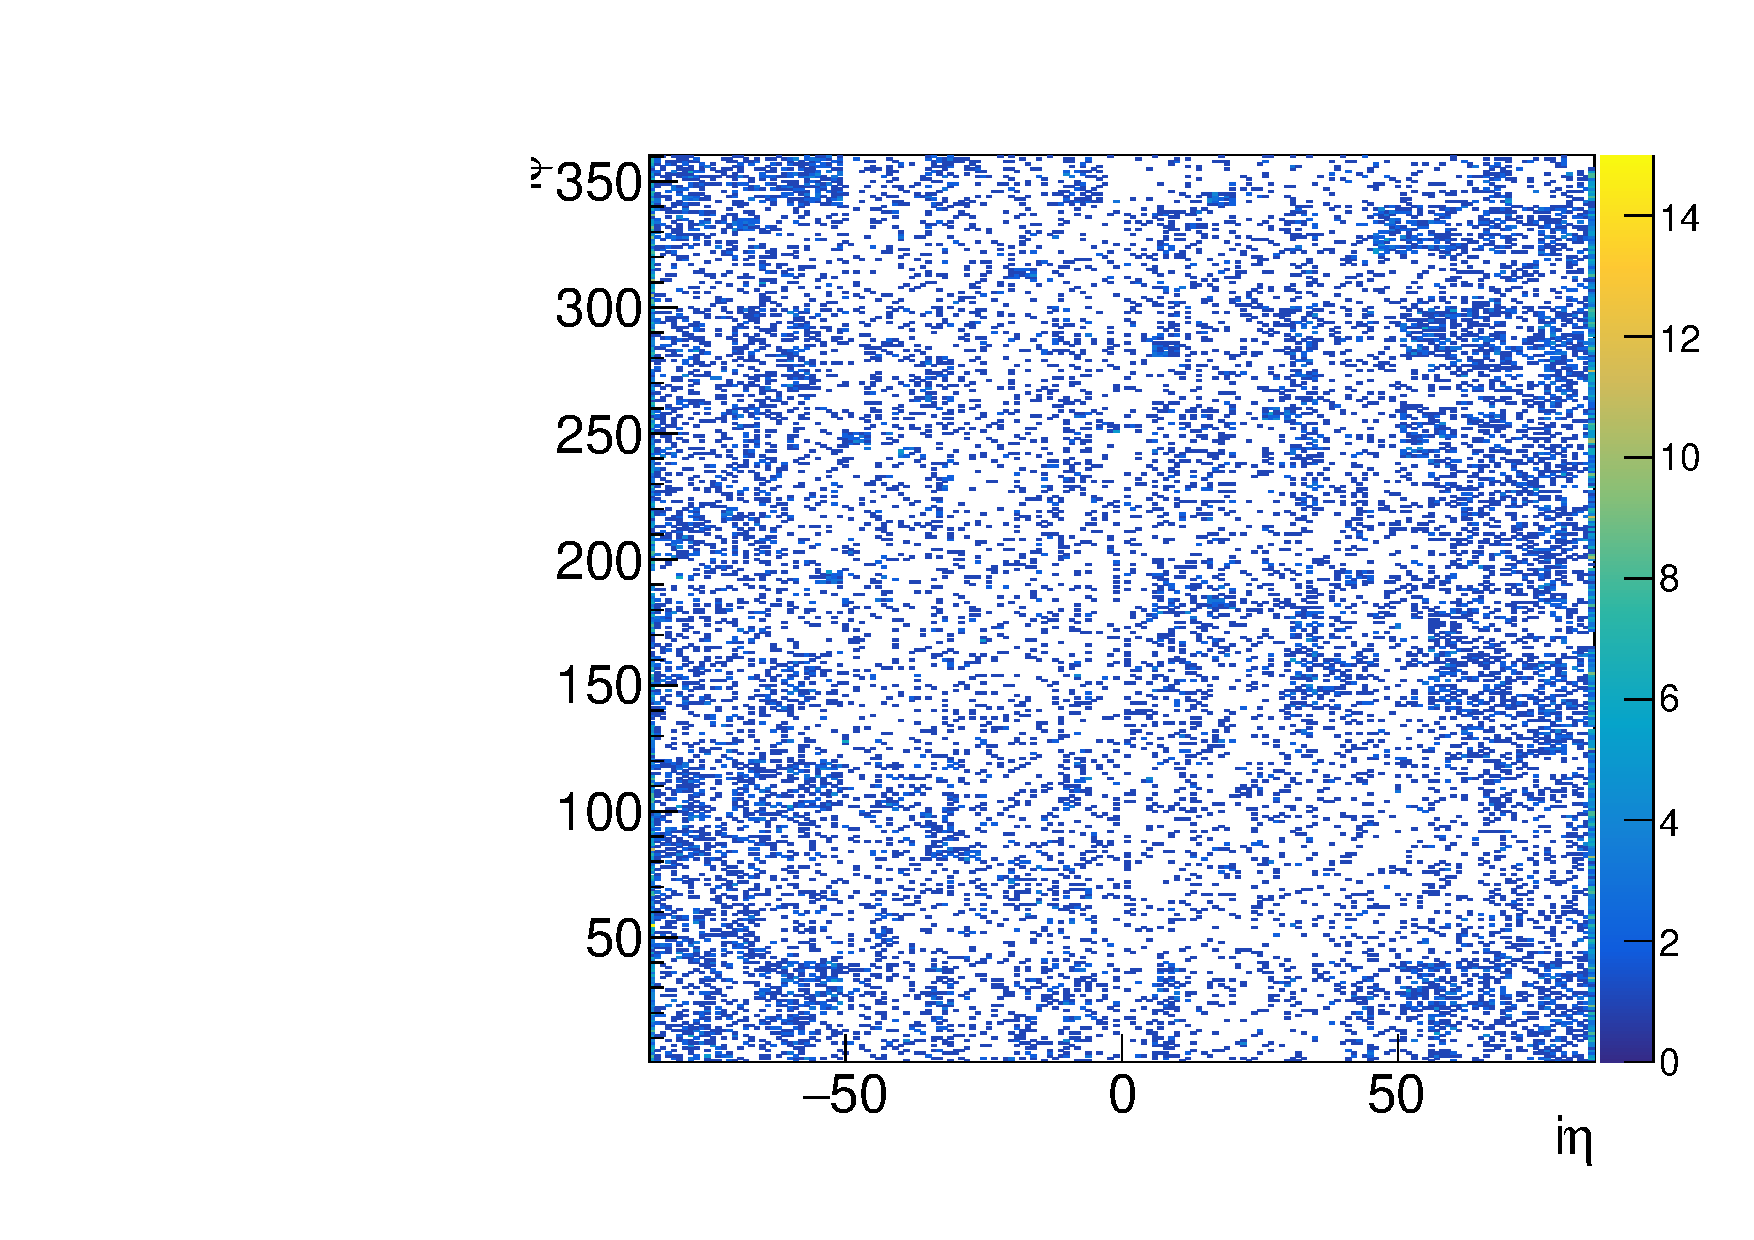
\includegraphics[width=0.45\textwidth]{Reconstruction/Figures/spikes/spike_map.pdf}
    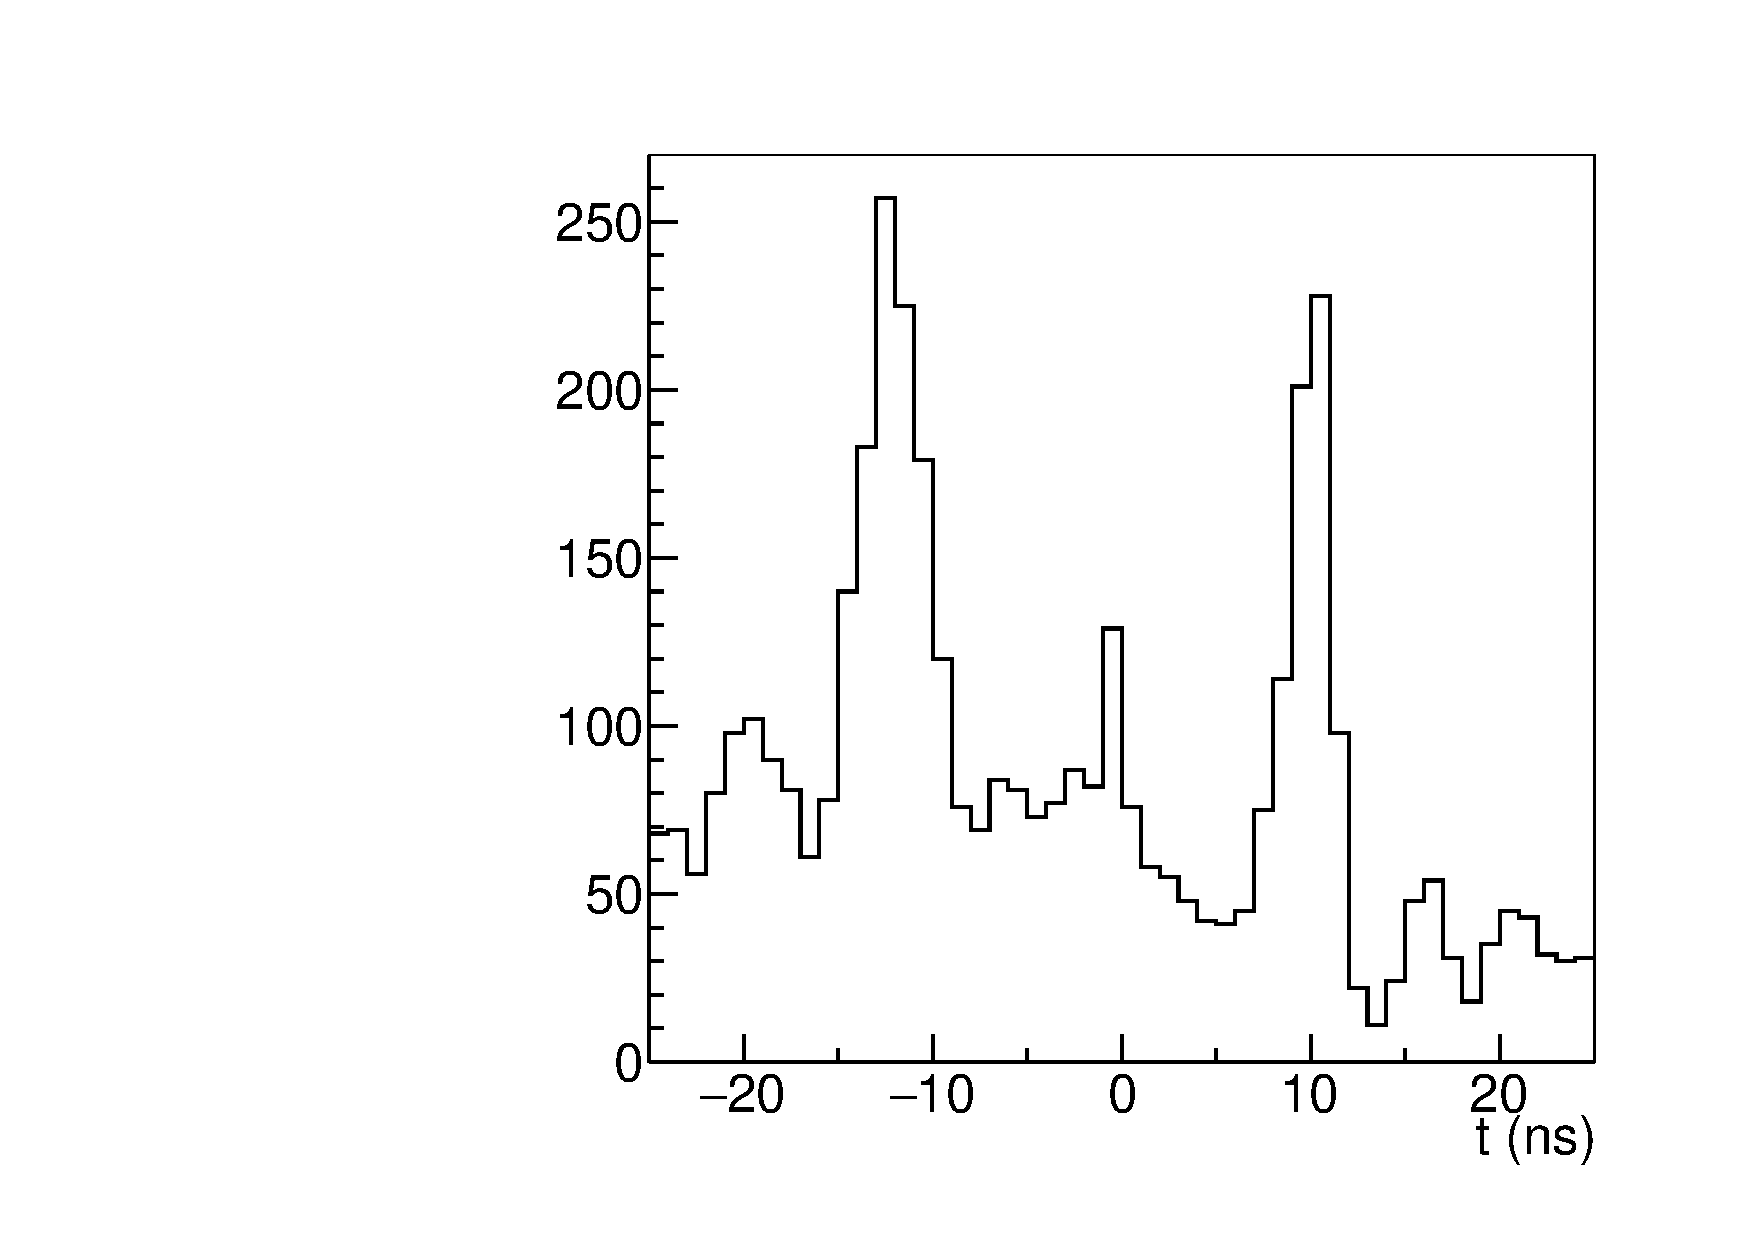
\includegraphics[width=0.45\textwidth]{Reconstruction/Figures/spikes/spike_time.pdf}
    \caption{
      $\eta$--$\phi$ and time distributions of seed hits of narrow ($\sieie < 0.001$) clusters.
    }
    \label{fig:spike_distributions}
  \end{center}
\end{figure}

Figure~\ref{fig:spike_distributions} shows the spacial and temporal distributions of the rec hits seeding narrow ($\sieie < 0.001$) clusters. 
The spacial distribution appears mostly random, indicating that there is no single source of spike-like rec hits. 
The two highest peaks in the time distribution at $t \sim -15\ns$ and $t \sim 10\ns$ are characteristic of pulse shapes, which rise faster than the pulse from the normal scintillation. 
The second peak is understood to come from the next bunch crossing.

\begin{figure}[tbp]
  \begin{center}
    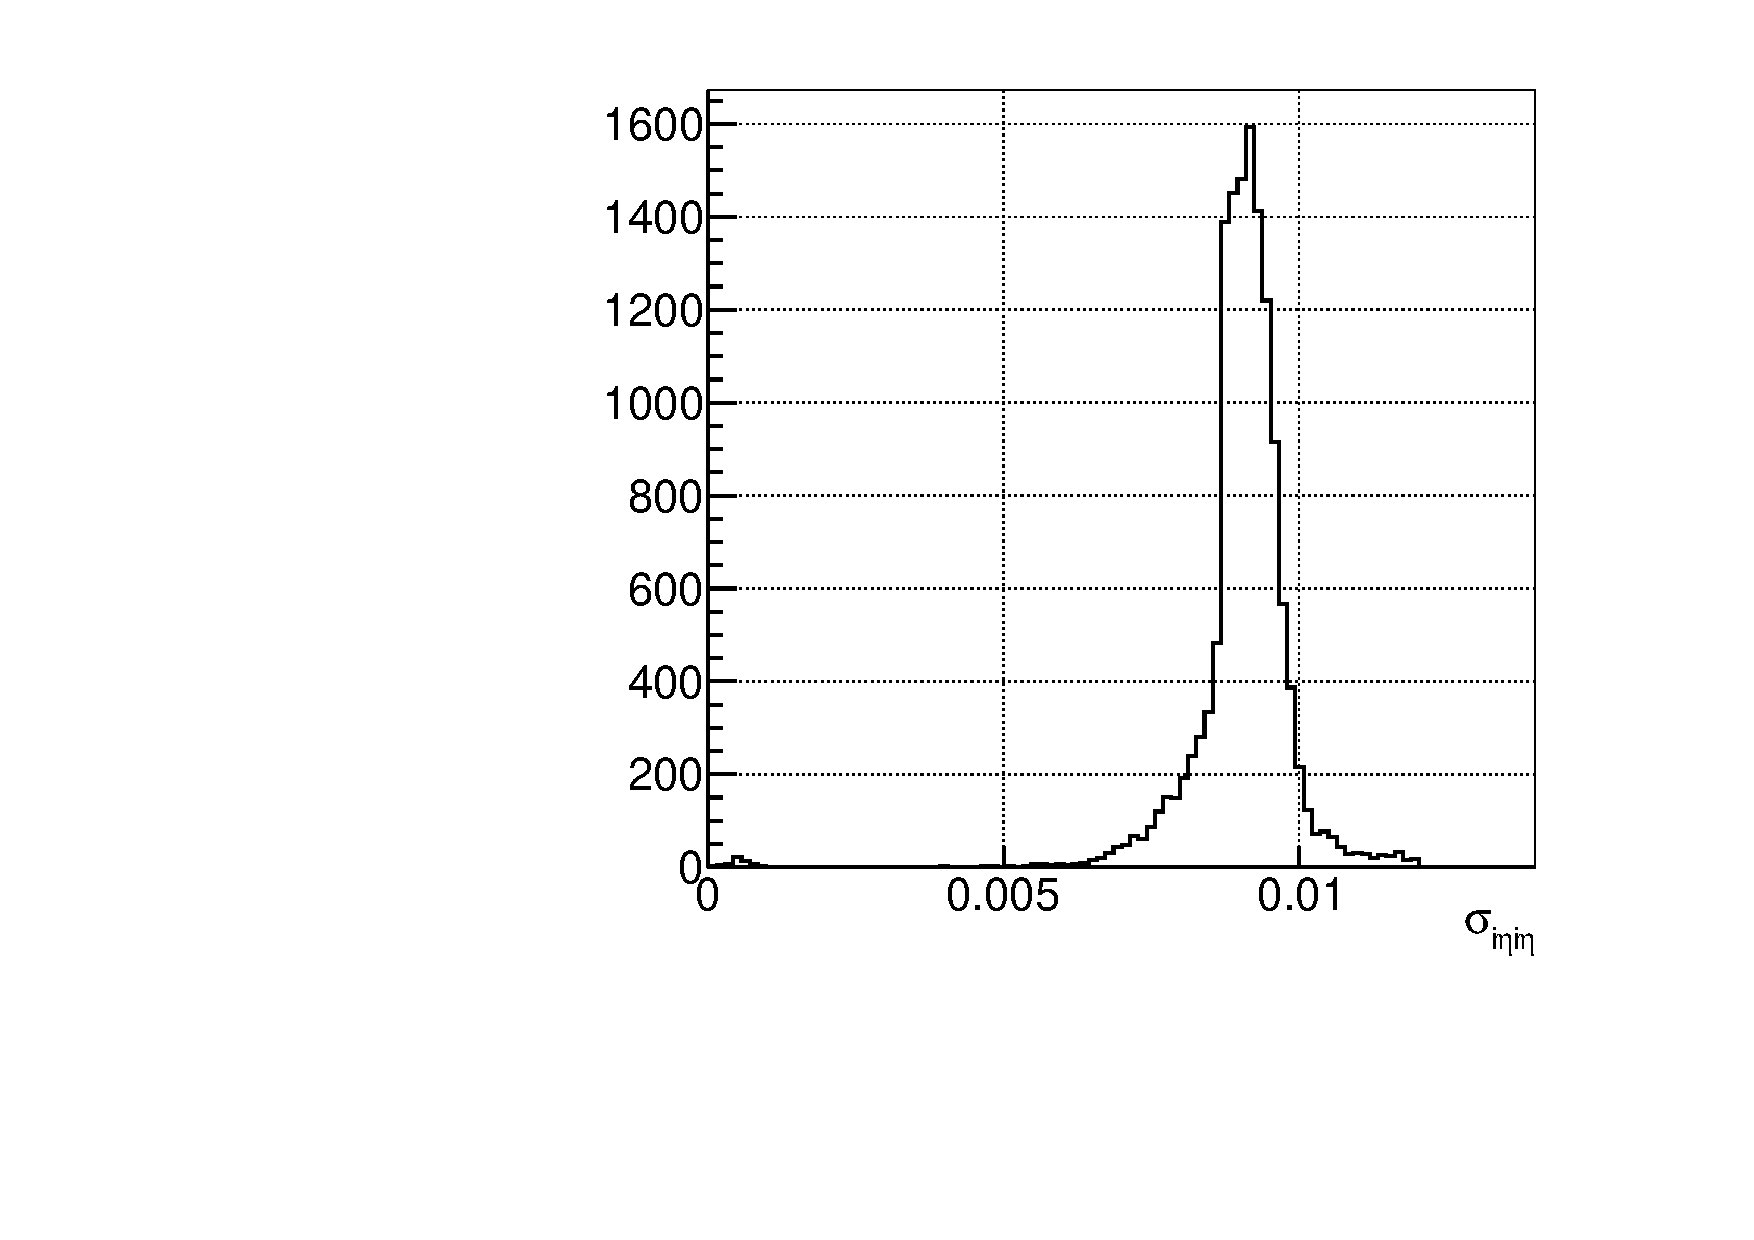
\includegraphics[width=0.45\textwidth]{Reconstruction/Figures/spikes/sieie_mc.pdf}
    \caption{
      \sieie distribution of uncleaned clusters from \gj\ MC simulation.
    }
    \label{fig:sieie_mc}
  \end{center}
\end{figure}

The small peak at $t\sim 0$ in the time distribution of Fig.~\ref{fig:spike_distributions} is due to actual ``physical'' clusters that happened to have a very narrow cluster shape. 
By processing the \gj\ MC simulation events through this special reconstruction, we see that about 0.5\% of ECAL clusters from prompt photons have $\sieie < 0.001$ as shown in Figure~\ref{fig:sieie_mc}.

\begin{figure}[tbp]
  \begin{center}
    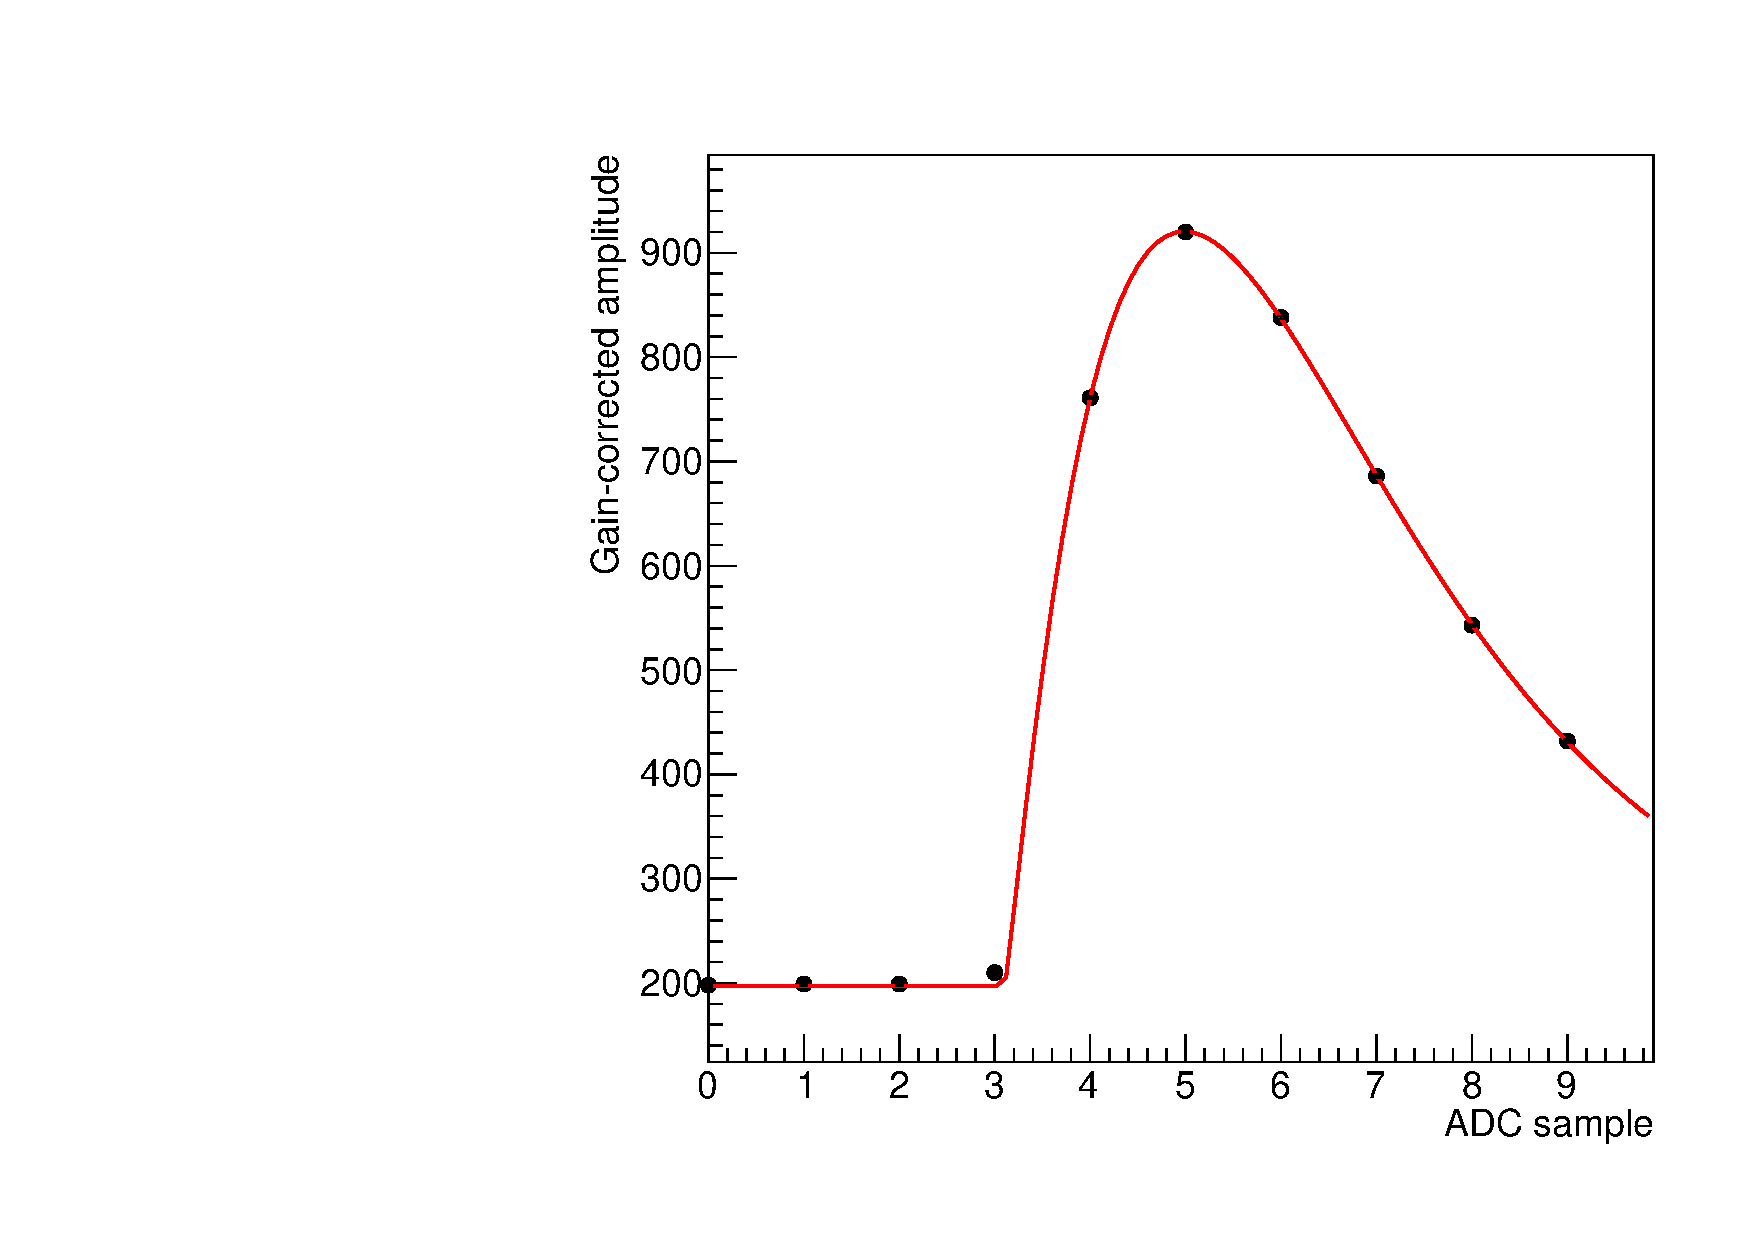
\includegraphics[width=0.3\textwidth]{Reconstruction/Figures/spikes/pulse_example_normal.pdf}
    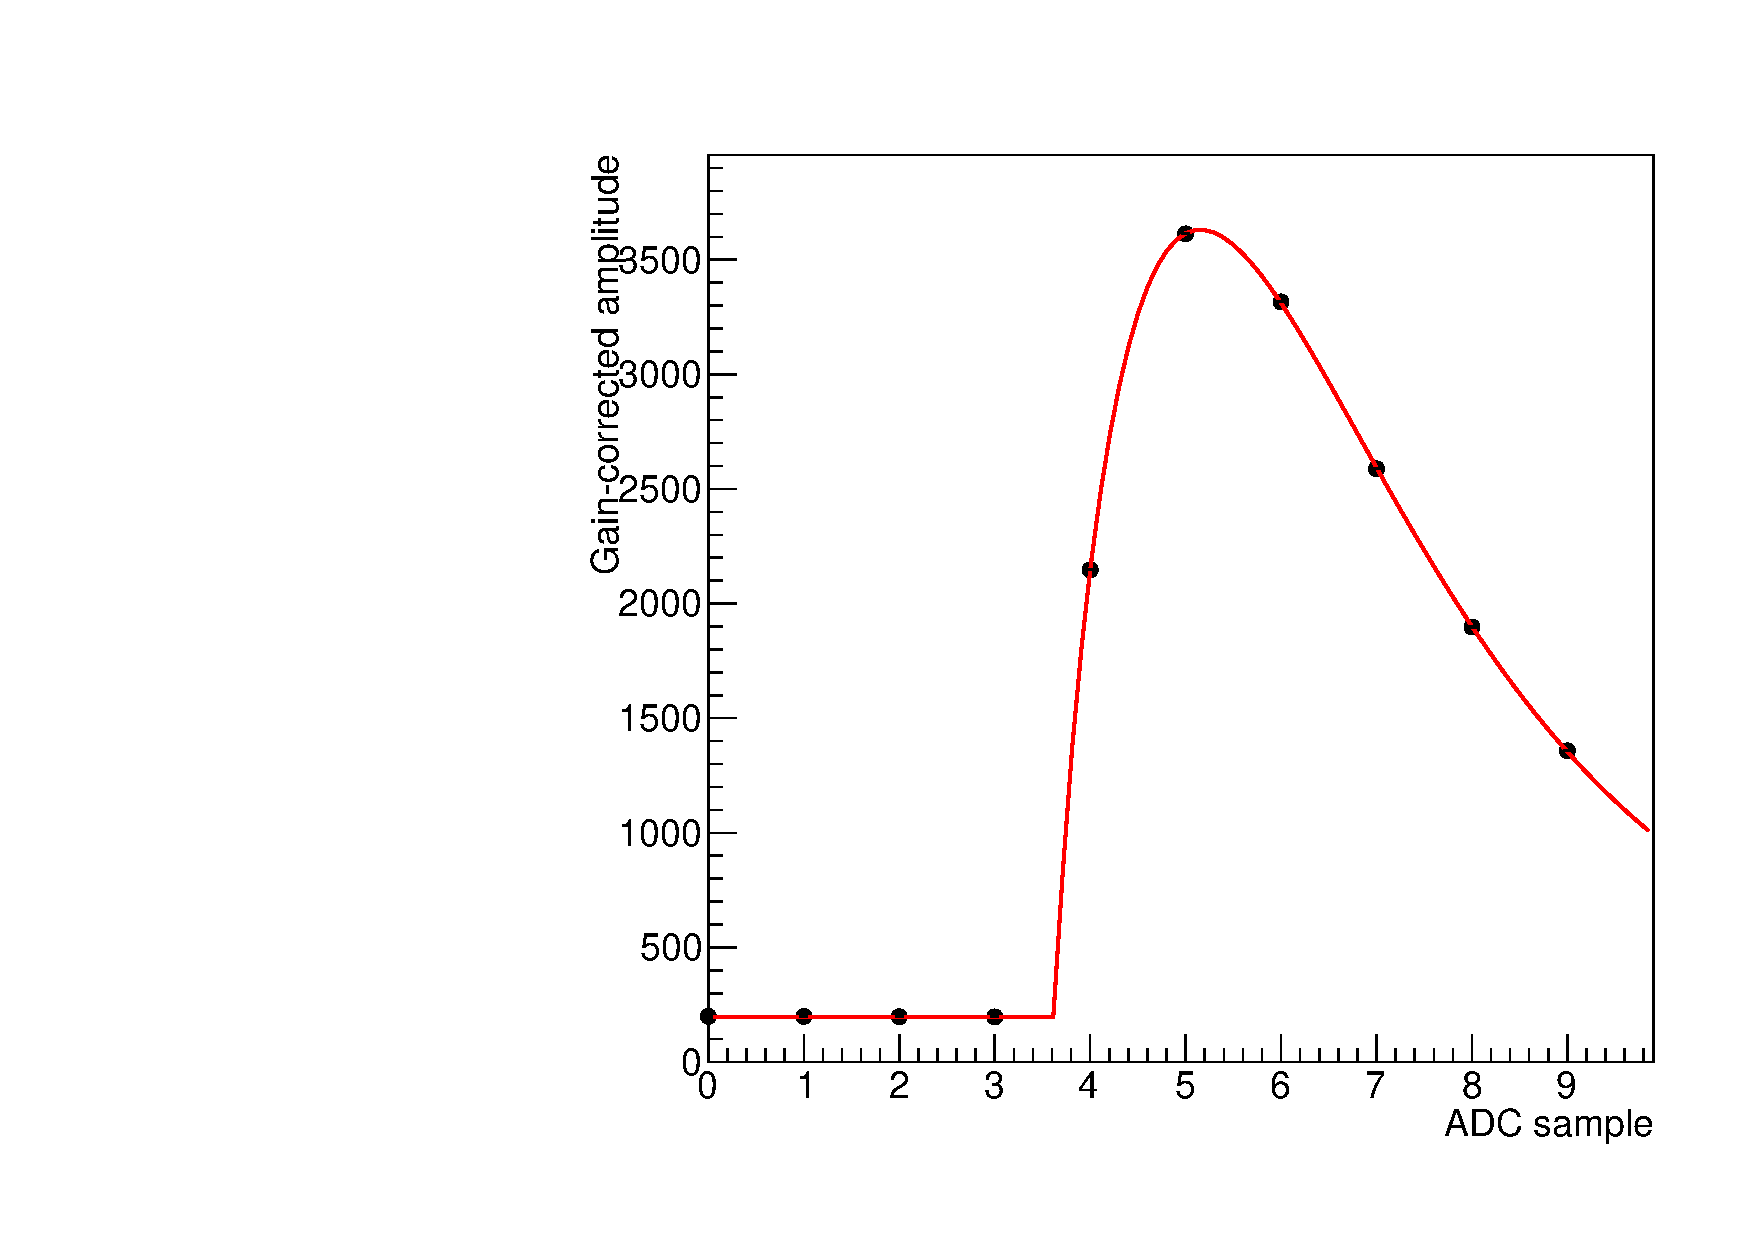
\includegraphics[width=0.3\textwidth]{Reconstruction/Figures/spikes/pulse_example_spike.pdf}
    \caption{
      Example ECAL DIGIs and corresponding pulse shapes reconstructed through $\chi^{2}$ fits of Equation~\ref{eqn:pulse_shape}, for normal (left) and spike-like (right) hits.
    }
    \label{fig:pulse_examples}
  \end{center}
\end{figure}

To understand the time distribution, one can investigate the original DIGI samples from which rec hits are made. 
At each event readout, a single ECAL channel outputs 10 ADC signals corresponding to a sampling of the analog pulse output of multi-gain preamplifier (MGPA) in range $t_{0} - 125\ns < t < t_{0} + 100\ns$, where $t_{0}$ is the time of the triggering bunch crossing. 
These 10 signal points can be described well by the formula

\begin{equation} \label{eqn:pulse_shape}
  f(t) = A \left(1 - \frac{t - \tau}{\alpha\beta}\right)^{\alpha} \exp \left(-\frac{t-\tau}{\beta}\right).
\end{equation}

\begin{figure}[tbp]
  \begin{center}
    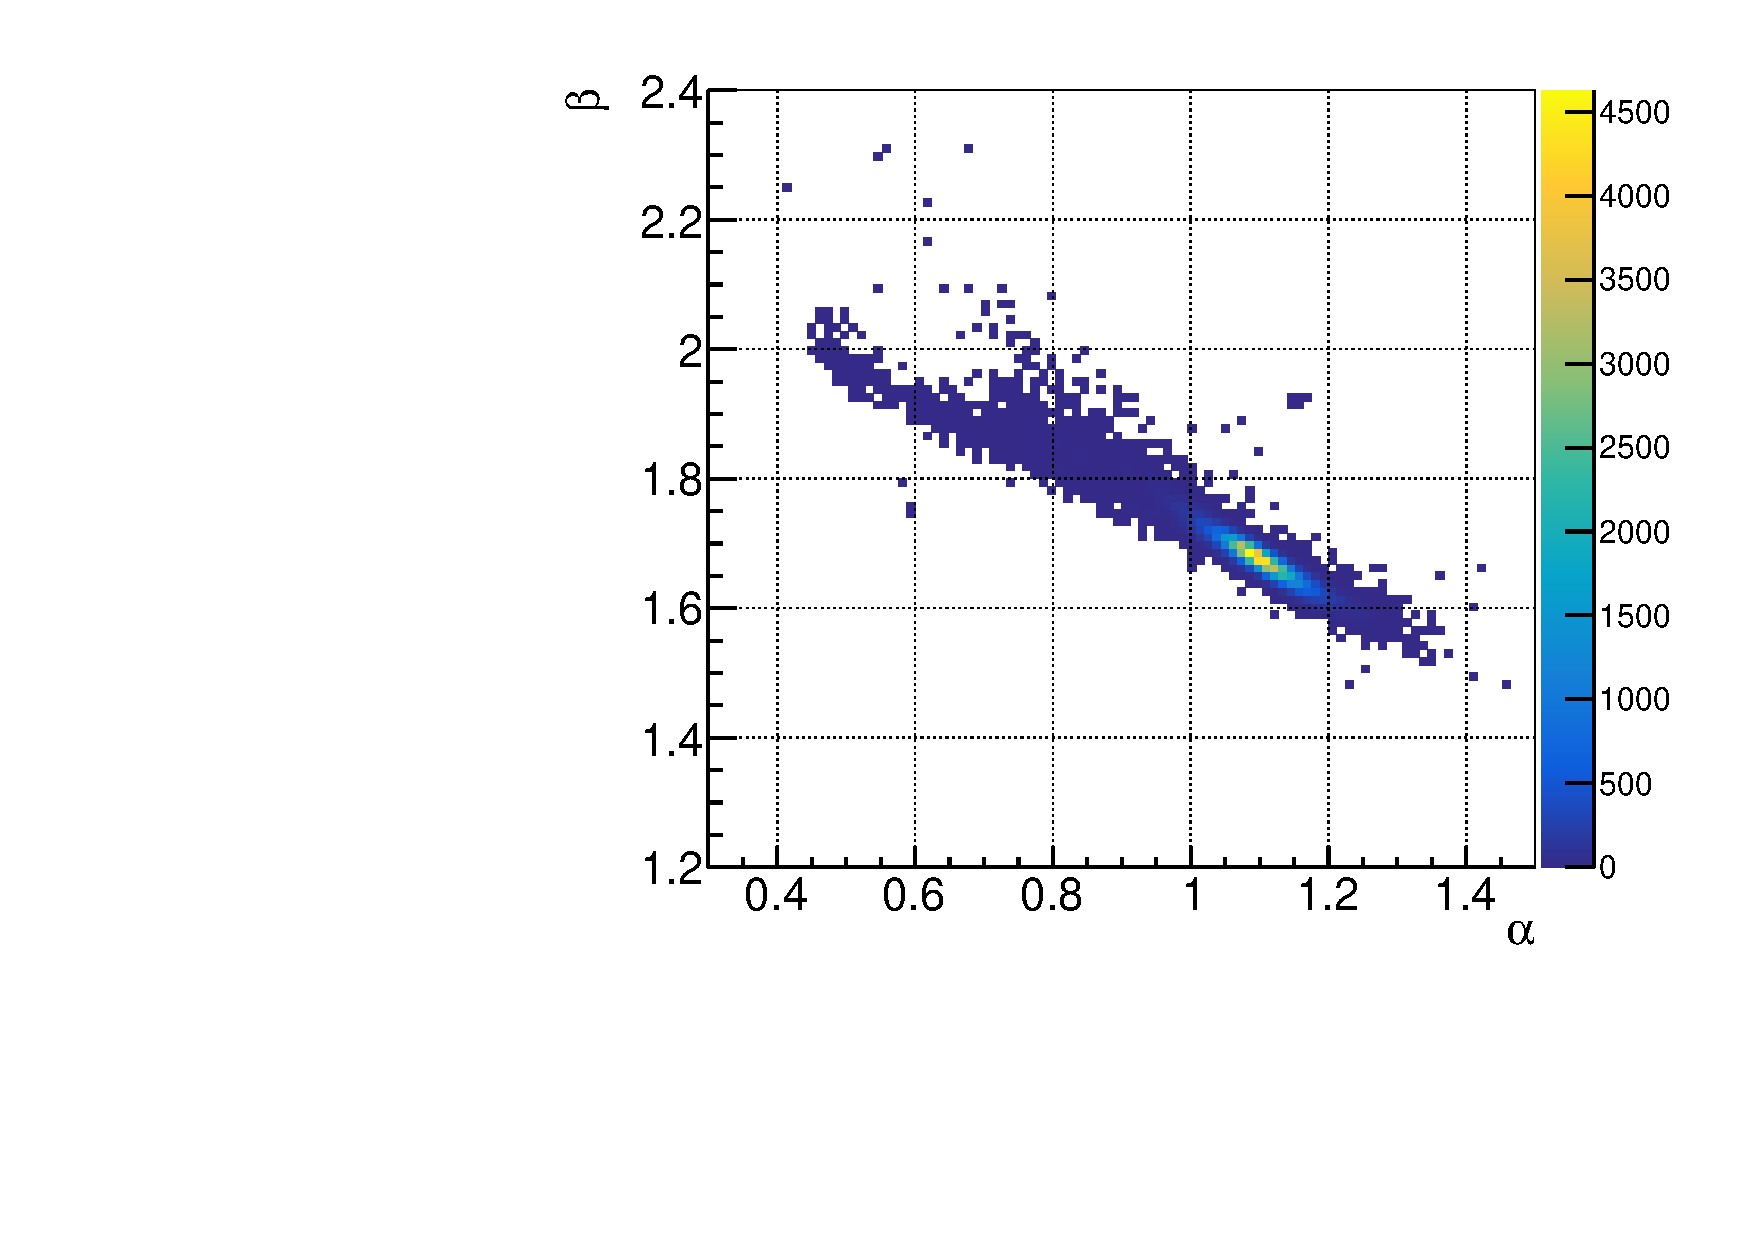
\includegraphics[width=0.45\textwidth]{Reconstruction/Figures/spikes/alphabeta_physical.pdf}
    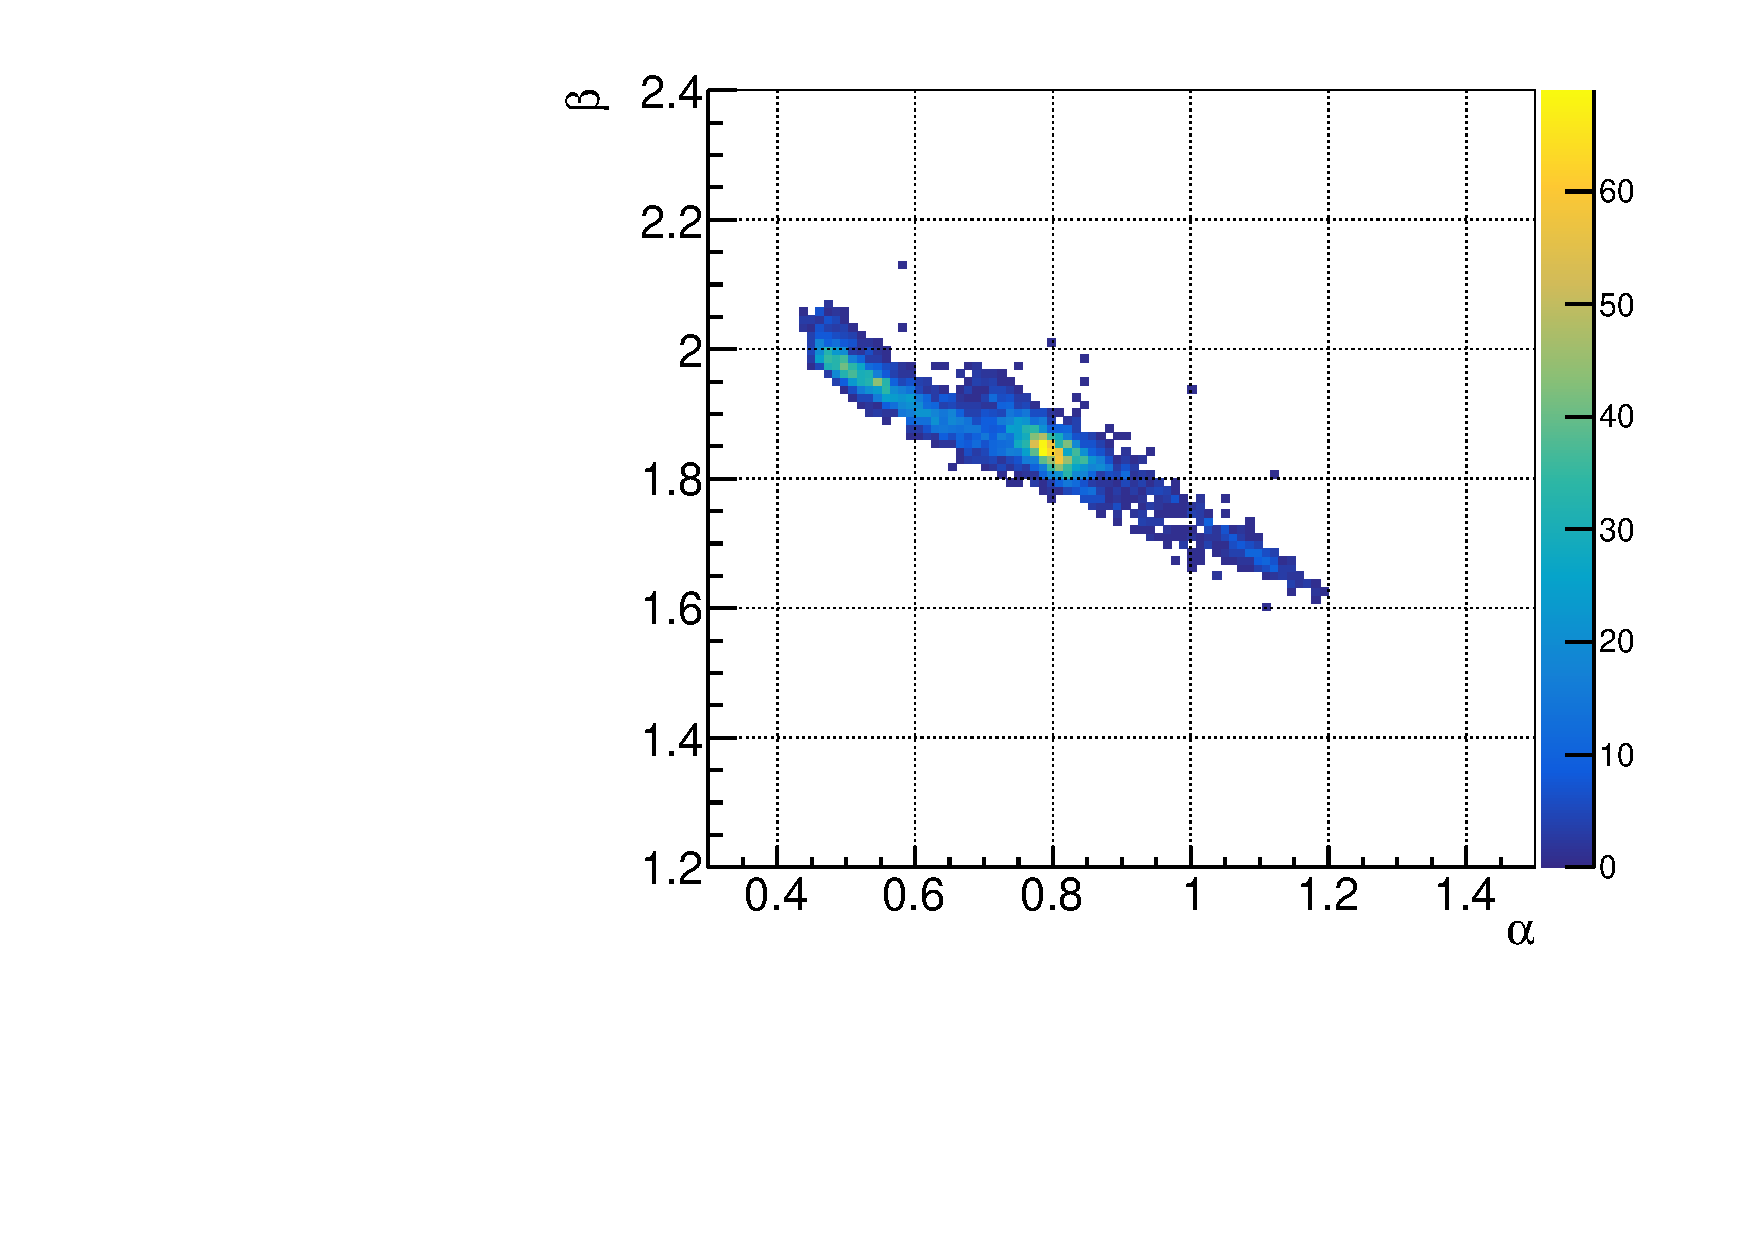
\includegraphics[width=0.45\textwidth]{Reconstruction/Figures/spikes/alphabeta_spike.pdf}
    \caption{
      $\alpha$--$\beta$ distributions of the seed hits of physical wide clusters (left) and spike-like clusters (right).
    }
    \label{fig:spike_alphabeta}
  \end{center}
\end{figure}

In the formula, parameters $A$ and $\tau$ correspond to the pulse amplitude and peak time, whereas $\alpha$ and $\beta$ control the shape of the pulse. 
Figure~\ref{fig:pulse_examples} illustrates various observed pulse shapes fit with the above formula with all parameters floating. 
A $\chi^{2}$ fit is employed using the average noise amplitude of each MGPA channel as the errors on the data points. 
The noise is measured in ECAL calibration cycles in the inter-fill period and is recorded in the conditions database.

\begin{figure}[tbp]
  \begin{center}
    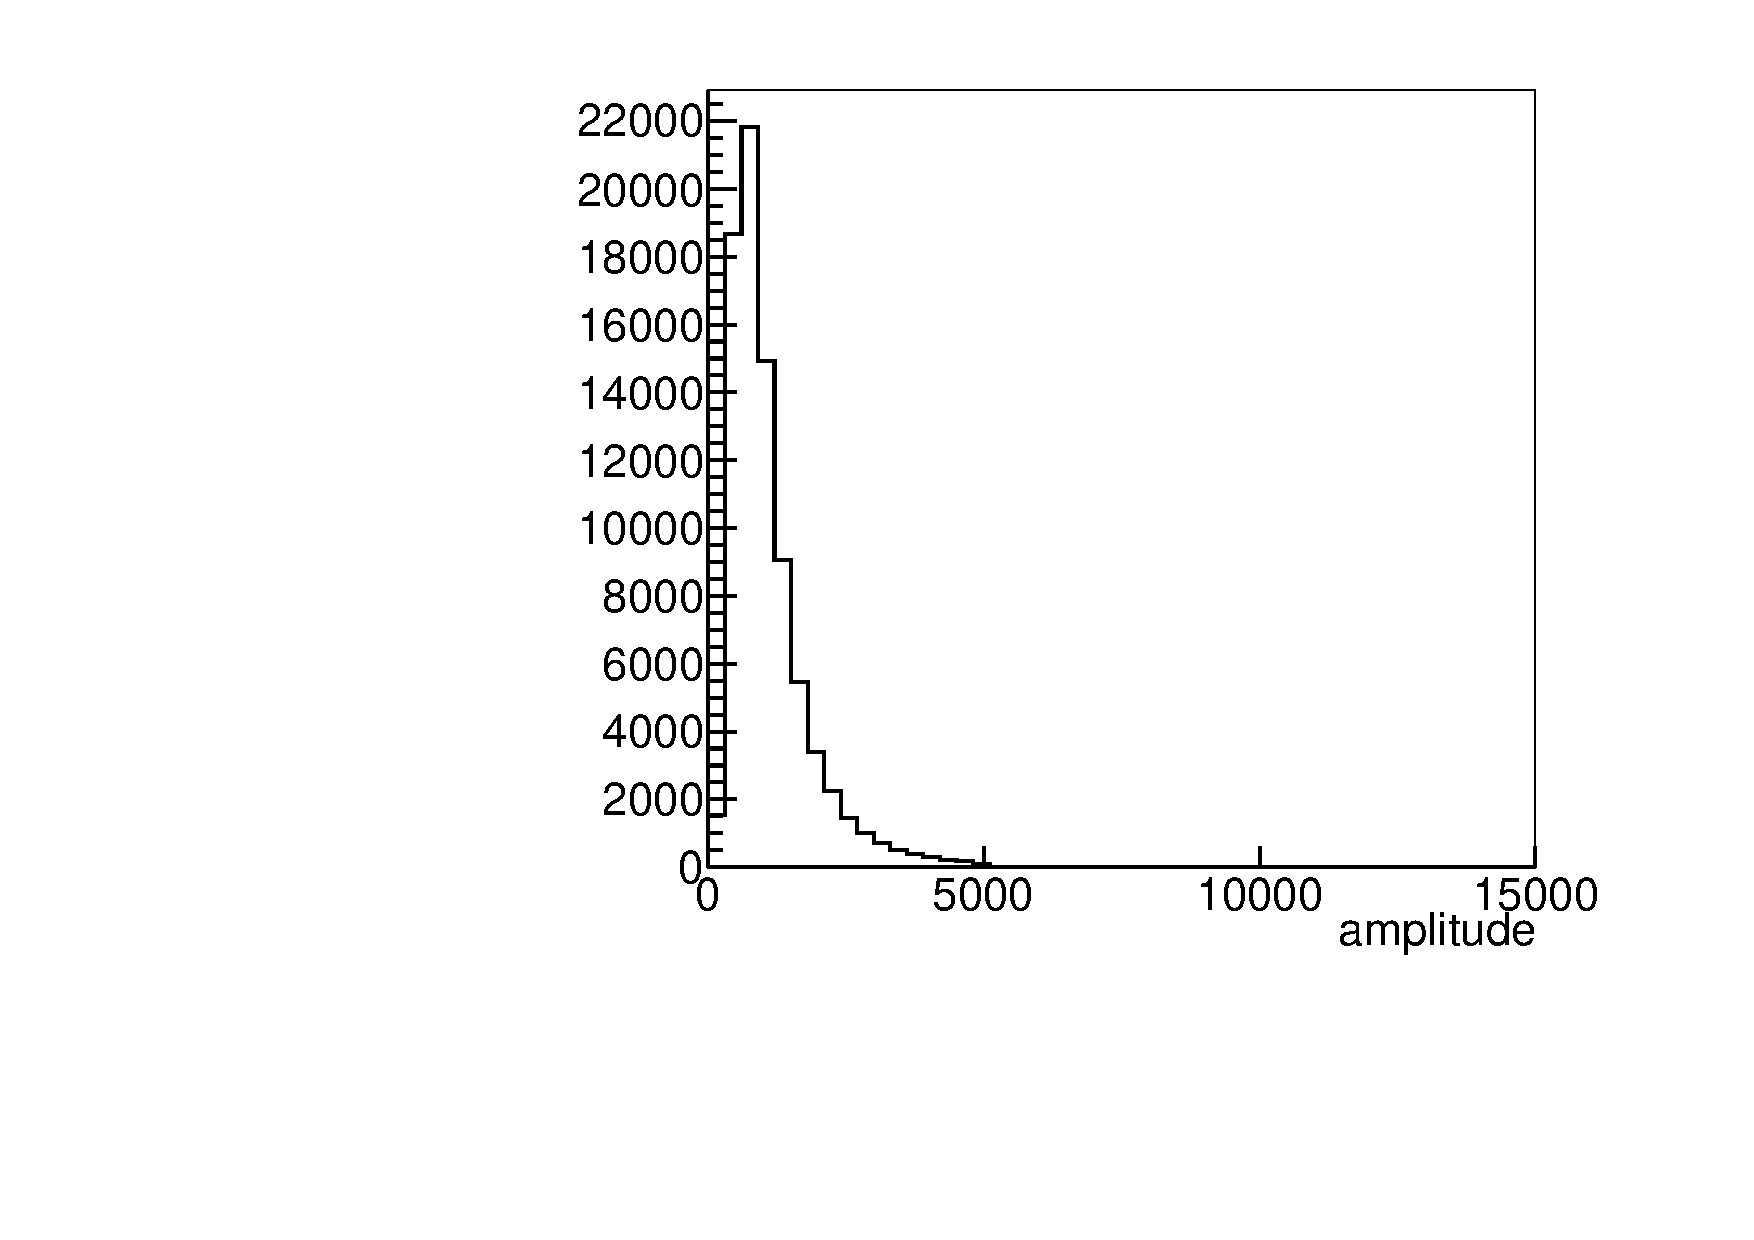
\includegraphics[width=0.3\textwidth]{Reconstruction/Figures/spikes/physical_amplitude.pdf}
    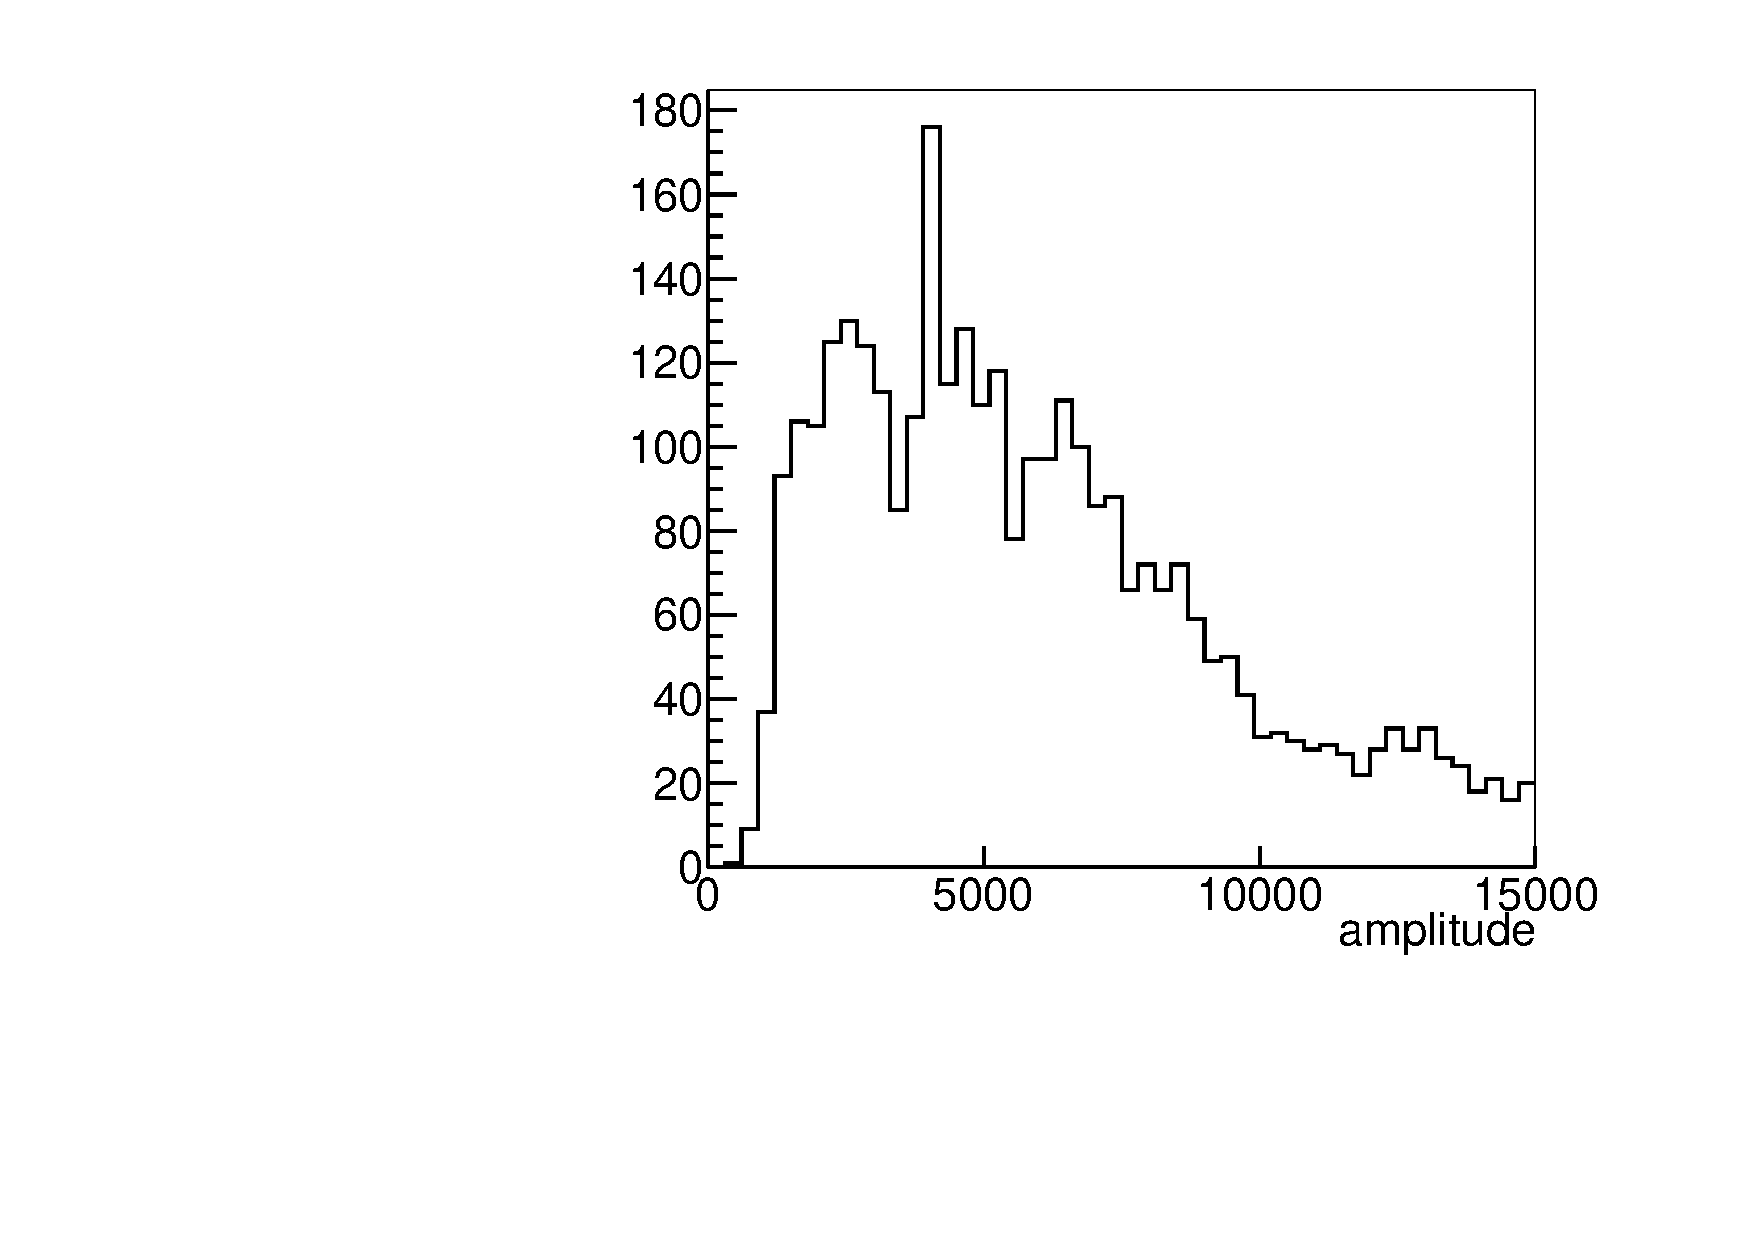
\includegraphics[width=0.3\textwidth]{Reconstruction/Figures/spikes/spike_amplitude.pdf}
    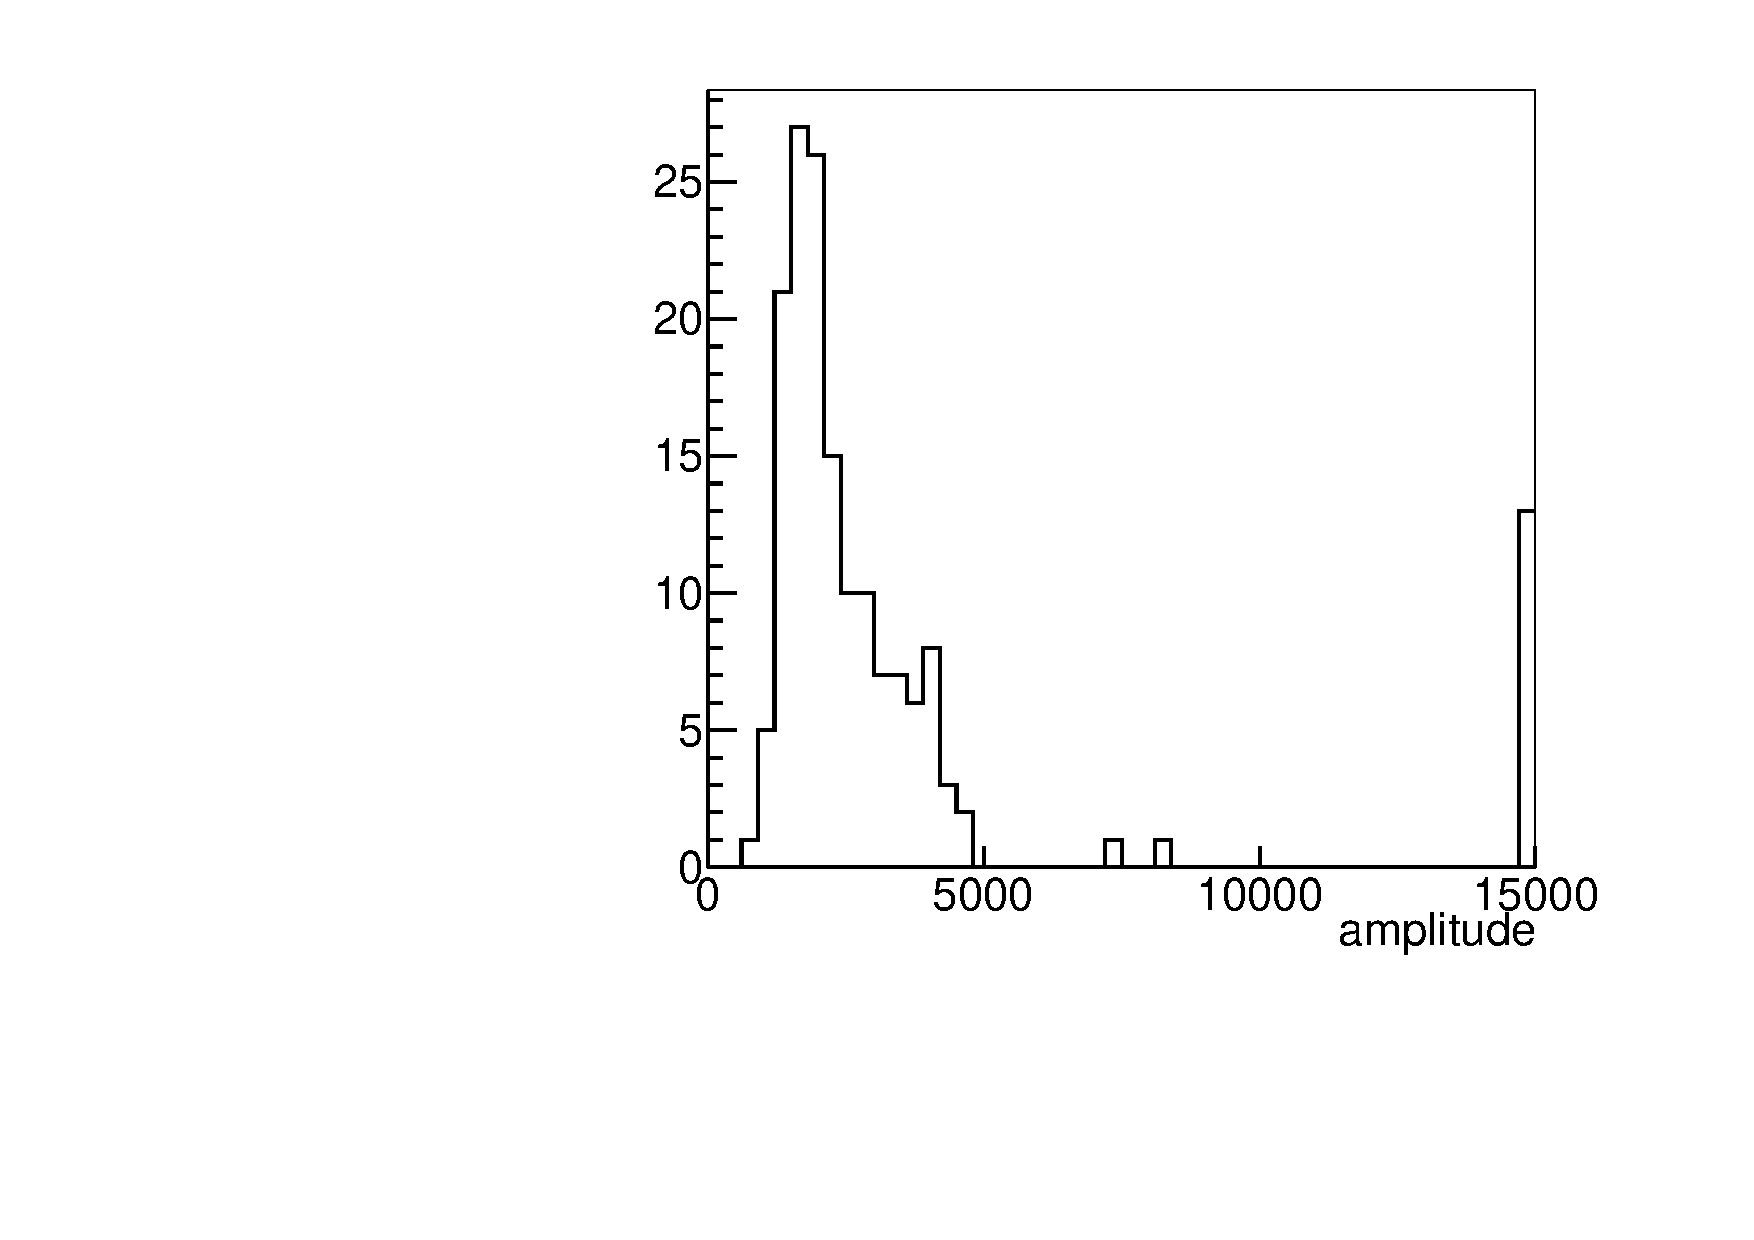
\includegraphics[width=0.3\textwidth]{Reconstruction/Figures/spikes/narrow_largealpha_amplitude.pdf}
    \caption{
      Seed crystal pulse amplitude distributions of physical wide clusters (left), narrow clusters with $\alpha < 0.9$ (center), and narrow clusters with $\alpha > 0.9$ (right).
    }
    \label{fig:spike_amplitudes}
  \end{center}
\end{figure}

In the $\alpha$--$\beta$ parameter space, seed rec hits of wide clusters concentrate around $(\alpha, \beta) \sim (1.1, 1.7)$, while spike-like hits populate the region $\alpha < 0.9$ as shown in Figure~\ref{fig:spike_alphabeta}.
In fact, the pulse amplitude distribution of narrow-cluster seeds with $\alpha > 0.9$ is unlike that of the narrow-cluster seeds with $\alpha < 0.9$, and resembles the amplitude distribution of wide-cluster seeds shown in Figure~\ref{fig:spike_amplitudes}.
This suggests that the population $\alpha > 0.9$ correspond to the clusters of physical, prompt photons.
It then follows that spike hits can be regarded to exclusively have sharp pulse shapes.
\fi
